\chapter{Introduction to data}
\label{introductionToData}

%\begin{tipBox}{\tipBoxTitle[Chapter Goal:]{Thinking about data}
%Understand basics about data organization, data types, numerical summaries of data, graphical summaries of data, and foundational techniques for data collection. We begin and end the chapter with case studies.}
%\end{tipBox}

Scientists seek to answer questions using rigorous methods and careful observations. These observations -- collected from the likes of field notes, surveys, and experiments -- form the backbone of a statistical investigation and are called \term{data}. Statistics is the study of how best to collect, analyze, and draw conclusions from data. It is helpful to put statistics in the context of a general process of investigation:
\begin{enumerate}
\setlength{\itemsep}{0mm}
\item Identify a question or problem.
\item Collect relevant data on the topic.
\item Analyze the data.
\item Form a conclusion.
%\item Make decisions based on the conclusion.
\end{enumerate}
Statistics as a subject focuses on making stages 2-4 objective, rigorous, and efficient. That~is, statistics has three primary components: How best can we collect data? How should it be analyzed? And what can we infer from the analysis?

The topics scientists investigate are as diverse as the questions they ask. However, many of these investigations can be addressed with a small number of data collection techniques, analytic tools, and fundamental concepts in statistical inference. This chapter provides a glimpse into these and other themes we will encounter throughout the rest of the book. We introduce the basic principles of each branch and learn some tools along the way. We will encounter applications from other fields, some of which are not typically associated with science but nonetheless can benefit from statistical study.

\section[Case study: using stents to prevent strokes]{Case study: using stents to prevent strokes \sectionvideohref{youtube-nEHFF1ADpWE&list=PLkIselvEzpM6pZ76FD3NoCvvgkj_p-dE8}}
\label{basicExampleOfStentsAndStrokes}

\index{data!stroke|(}

Section~\ref{basicExampleOfStentsAndStrokes} introduces a classic challenge in statistics: evaluating the efficacy of a medical treatment. Terms in this section, and indeed much of this chapter, will all be revisited later in the text. The plan for now is simply to get a sense of the role statistics can play in practice.

In this section we will consider an experiment that studies effectiveness of stents in treating patients at risk of stroke.\footnote{Chimowitz MI, Lynn MJ, Derdeyn CP, et al. 2011. Stenting versus Aggressive Medical Therapy for Intracranial Arterial Stenosis. New England Journal of Medicine 365:993-1003. \oiRedirect{textbook-nejm_stent_study}{www.nejm.org/doi/full/10.1056/NEJMoa1105335}. NY Times article reporting on the study: \oiRedirect{textbook-nytimes_stent_study}{www.nytimes.com/2011/09/08/health/research/08stent.html}.} Stents are devices put inside blood vessels that assist in patient recovery after cardiac events and reduce the risk of an additional heart attack or death. Many doctors have hoped that there would be similar benefits for patients at risk of stroke. We start by writing the principal question the researchers hope to answer:
\begin{quote}
Does the use of stents reduce the risk of stroke?
\end{quote}

The researchers who asked this question collected data on 451 at-risk patients. Each volunteer patient was randomly assigned to one of two groups:
\begin{itemize}
\item[]\termsub{Treatment group}{treatment group}. Patients in the treatment group received a stent and medical management. The medical management included medications, management of risk factors, and help in lifestyle modification.
\item[]\termsub{Control group}{control group}. Patients in the control group received the same medical management as the treatment group, but they did not receive stents.
\end{itemize}
Researchers randomly assigned 224 patients to the treatment group and 227 to the control group. In this study, the control group provides a reference point against which we can measure the medical impact of stents in the treatment group.

Researchers studied the effect of stents at two time points: 30~days after enrollment and 365~days after enrollment. The results of 5 patients are summarized in Table~\ref{stentStudyResultsDF}. Patient outcomes are recorded as ``stroke'' or ``no event'', representing whether or not the patient had a stroke at the end of a time period.

\begin{table}[h]
\centering
\begin{tabular}{l ccc}
\hline
Patient	&	group	&	0-30 days 	&	0-365 days \\
\hline
1		&	treatment &	no event &	no event \\
2		&	treatment &	stroke & stroke \\
3		&	treatment &	no event & no event \\
$\vdots$	&	$\vdots$	  &	$\vdots$ \\
450	&	control &	no event &	no event \\
451	&	control &	no event &	no event \\
\hline
\end{tabular}
\caption{Results for five patients from the stent study.}
\label{stentStudyResultsDF}
% trmt <- c(rep('trmt', 224), rep('control', 227)); outcome30 <- c(rep(c('event', 'no_event'), c(33, 191)), rep(c('event', 'no_event'), c(13, 214))); outcome365 <- c(rep(c('event', 'no_event'), c(33, 191)), rep(c('event', 'no_event'), c(13, 214)))
\end{table}

Considering data from each patient individually would be a long, cumbersome path towards answering the original research question. Instead, performing a statistical data analysis allows us to consider all of the data at once. Table~\ref{stentStudyResults} summarizes the raw data in a more helpful way. In this table, we can quickly see what happened over the entire study. For instance, to identify the number of patients in the treatment group who had a stroke within 30 days, we look on the left-side of the table at the intersection of the treatment and stroke: 33.

\begin{table}[h]
\centering
\begin{tabular}{l cc c cc}
& \multicolumn{2}{c}{0-30 days} &\hspace{5mm}\ & \multicolumn{2}{c}{0-365 days} \\
  \cline{2-3} \cline{5-6}
	& 	stroke 	& no event && 	stroke 	& no event \\
  \hline
treatment 	& 33		& 191	&&	45 	& 179 \\
control 		& 13		& 214	&& 	28	& 199 \\
  \hline
Total				& 46		& 405	&&	73	& 378 \\
  \hline
\end{tabular}
\caption{Descriptive statistics for the stent study.}
\label{stentStudyResults}
\end{table}

\begin{exercise}
Of the 224 patients in the treatment group, 45 had a stroke by the end of the first year. Using these two numbers, compute the proportion of patients in the treatment group who had a stroke by the end of their first year. (Please note: answers to all in-text exercises are provided using footnotes.)\footnote{The proportion of the 224 patients who had a stroke within 365 days: $45/224 = 0.20$.}
\end{exercise}

We can compute summary statistics from the table. A \term{summary statistic} is a single number summarizing a large amount of data.\footnote{Formally, a summary statistic is a value computed from the data. Some summary statistics are more useful than others.} For instance, the primary results of the study after 1~year could be described by two summary statistics: the proportion of people who had a stroke in the treatment and control groups.
\begin{itemize}
\setlength{\itemsep}{0mm}
\item[] Proportion who had a stroke in the treatment (stent) group: $45/224 = 0.20 = 20\%$.
\item[] Proportion who had a stroke in the control group: $28/227 = 0.12 = 12\%$.
\end{itemize}
These two summary statistics are useful in looking for differences in the groups, and we are in for a surprise: an additional 8\% of patients in the treatment group had a stroke! This is important for two reasons. First, it is contrary to what doctors expected, which was that stents would \emph{reduce} the rate of strokes. Second, it leads to a statistical question: do the data show a ``real'' difference between the groups?

This second question is subtle. Suppose you flip a coin 100 times. While the chance a coin lands heads in any given coin flip is 50\%, we probably won't observe exactly 50 heads. This type of fluctuation is part of almost any type of data generating process. It is possible that the 8\% difference in the stent study is due to this natural variation. However, the larger the difference we observe (for a particular sample size), the less believable it is that the difference is due to chance. So what we are really asking is the following: is the difference so large that we should reject the notion that it was due to chance?

While we don't yet have our statistical tools to fully address this question on our own, we can comprehend the conclusions of the published analysis: there was compelling evidence of harm by stents in this study of stroke patients.

\textbf{Be careful:} do not generalize the results of this study to all patients and all stents. This study looked at patients with very specific characteristics who volunteered to be a part of this study and who may not be representative of all stroke patients. In addition, there are many types of stents and this study only considered the self-expanding Wingspan stent (Boston Scientific). However, this study does leave us with an important lesson: we should keep our eyes open for surprises.

\index{data!stroke|)}

\section[Data basics]{Data basics \sectionvideohref{youtube-Mjif8PTgzUs&list=PLkIselvEzpM6pZ76FD3NoCvvgkj_p-dE8}}
\label{dataBasics}

Effective presentation and description of data is a first step in most analyses. This section introduces one structure for organizing data as well as some terminology that will be used throughout this book.

\subsection{Observations, variables, and data matrices}

\index{data!email50|(}

Table~\ref{email50DF} displays rows 1, 2, 3, and 50 of a data set concerning 50 emails received during early 2012. These observations will be referred to as the \data{email50} data set, and they are a random sample from a larger data set that we will see in Section~\ref{categoricalData}.

Each row in the table represents a single email or \term{case}.\footnote{A case is also sometimes called a \term{unit of observation} or an \term{observational unit}.} The columns represent characteristics, called \termsub{variables}{variable}, for each of the emails. For example, the first row represents email 1, which is a not spam, contains 21,705 characters, 551 line breaks, is written in HTML format, and contains only small numbers.

In practice, it is especially important to ask clarifying questions to ensure important aspects of the data are understood. For instance, it is always important to be sure we know what each variable means and the units of measurement. Descriptions of all five email variables are given in Table~\ref{email50Variables}.

\begin{table}[t]
\centering
\begin{tabular}{cc ccc c}
  \hline
 & \var{spam} & \var{num\_\hspace{0.3mm}char} & \var{line\_\hspace{0.3mm}breaks} & \var{format} & \var{number} \\ 
  \hline
1 & no & 21,705 & 551 & html & small \\ 
  2 & no & 7,011 & 183 & html & big \\ 
  3 & yes & 631 & 28 & text & none \\ 
$\vdots$ & $\vdots$ & $\vdots$ & $\vdots$ & $\vdots$ & $\vdots$ \\
  50 & no & 15,829 & 242 & html & small \\ 
   \hline
\end{tabular}
\caption{Four rows from the \data{email50} data matrix.}
\label{email50DF}
\end{table}
% library(openintro); library(xtable); data(email50); email50[c(1,2,3,50),c("spam", "num_char", "line_breaks", "format", "number")]; xtable(email50[c(1,2,3,50),c("spam", "num_char", "line_breaks", "format", "number")], digits=0)


\begin{table}[t]
\centering\small
\begin{tabular}{lp{10.5cm}}
\hline
{\bf variable} & {\bf description} \\
\hline
\var{spam} & Specifies whether the message was spam \\
\var{num\_\hspace{0.3mm}char} & The number of characters in the email   \\
\var{line\_\hspace{0.3mm}breaks} & The number of line breaks in the email (not including text wrapping)   \\
\var{format} & Indicates if the email contained special formatting, such as bolding, tables, or links, which would indicate the message is in HTML format    \\
\var{number} & Indicates whether the email contained no number, a small number (under 1 million), or a large number   \\
\hline
\end{tabular}
\caption{Variables and their descriptions for the \data{email50} data set.\textC{\vspace{-3.5mm}}}
\label{email50Variables}
\end{table}

\index{data!email50|)}

The data in Table~\ref{email50DF} represent a \term{data matrix}, which is a common way to organize data. Each row of a data matrix corresponds to a unique case, and each column corresponds to a variable. A data matrix for the stroke study introduced in Section~\ref{basicExampleOfStentsAndStrokes} is shown in Table~\vref{stentStudyResultsDF}, where the cases were patients and there were three variables recorded for each patient.

Data matrices are a convenient way to record and store data. If another individual or case is added to the data set, an additional row can be easily added. Similarly, another column can be added for a new variable.

\index{data!county|(}

\begin{exercise}
We consider a publicly available data set that summarizes information about the 3,143 counties in the United States, and we call this the \data{county} data set. This data set includes information about each county: its name, the state where it resides, its population in 2000 and 2010, per capita federal spending, poverty rate, and five additional characteristics. How might these data be organized in a data matrix? Reminder: look in the footnotes for answers to in-text exercises.\footnote{Each county may be viewed as a case, and there are eleven pieces of information recorded for each case. A table with 3,143 rows and 11 columns could hold these data, where each row represents a county and each column represents a particular piece of information.}
\end{exercise}

\noindent Seven rows of the \data{county} data set are shown in Table~\ref{countyDF}, and the variables are summarized in Table~\ref{countyVariables}. These data were collected from the US Census website.\footnote{\oiRedirect{textbook-census_quick_facts}{quickfacts.census.gov/qfd/index.html}}

\begin{landscape}
\begin{table}
\centering\small
\begin{tabular}{ccc ccc ccc ccc}
\hline
& \var{name} & \var{state} & \var{pop2000} & \var{pop2010} &
   \var{fed\_\hspace{0.3mm}spend} & \var{poverty} & \var{homeownership} & \var{multiunit} &
   \var{income} & \var{med\_\hspace{0.3mm}income} & \var{smoking\_\hspace{0.3mm}ban} \\
\hline
  1 & Autauga & AL & 43671 & 54571 & 6.068 & 10.6 & 77.5 & 7.2 & 24568 & 53255 & none \\
  2 & Baldwin & AL & 140415 & 182265 & 6.140 & 12.2 & 76.7 & 22.6 & 26469 & 50147 & none \\ 
  3 & Barbour & AL & 29038 & 27457 & 8.752 & 25.0 & 68.0 & 11.1 & 15875 & 33219 & none \\ 
  4 & Bibb & AL & 20826 & 22915 & 7.122 & 12.6 & 82.9 & 6.6 & 19918 & 41770 & none \\ 
  5 & Blount & AL & 51024 & 57322 & 5.131 & 13.4 & 82.0 & 3.7 & 21070 & 45549 & none \\ 
  $\vdots$ & $\vdots$ & $\vdots$ & $\vdots$ & $\vdots$ & $\vdots$ & $\vdots$ & $\vdots$ & $\vdots$ & $\vdots$ & $\vdots$ & $\vdots$ \\
  3142 & Washakie & WY & 8289 & 8533 & 8.714 & 5.6 & 70.9 & 10.0 & 28557 & 48379 & none \\ 
  3143 & Weston & WY & 6644 & 7208 & 6.695 & 7.9 & 77.9 & 6.5 & 28463 & 53853 & none \\ 
\hline
\end{tabular}
\caption{Seven rows from the \data{county} data set.}
\label{countyDF}
% library(openintro); county <- countyComplete[,c("name", "state", "pop2000", "pop2010", "fed_spending", "poverty", "home_ownership", "housing_multi_unit", "per_capita_income", "median_household_income")]; colnames(county) <- c("name", "state", "pop2000", "pop2010", "fed_spend", "poverty", "homeownership", "multiunit", "income", "med_income"); county$fed_spend <- county$fed_spend / county$pop2010

% library(openintro); library(xtable); cc <- countyComplete; xtable(cc[c(1:5,nrow(cc) - (1:0)), c("name", "state", "pop2000", "pop2010", "fed_spend", "poverty", "homeownership", "multiunit", "income", "med_income")], digits=1)
\end{table}

\begin{table}
\centering\small
\begin{tabular}{lp{11cm}}
\hline
{\bf variable} & {\bf description} \\
\hline
\var{name} & County name \\
\var{state} & State where the county resides (also including the District of Columbia) \\
\var{pop2000} & Population in 2000 \\
\var{pop2010} & Population in 2010 \\
\var{fed\_\hspace{0.3mm}spend} & Federal spending per capita \\
\var{poverty}  &  Percent of the population in poverty \\
\var{homeownership}  &  Percent of the population that lives in their own home or lives with the owner (e.g. children living with parents who own the home) \\
\var{multiunit}  &  Percent of living units that are in multi-unit structures (e.g. apartments) \\
\var{income} & Income per capita \\
\var{med\_\hspace{0.3mm}income} & Median household income for the county, where a household's income equals the total income of its occupants who are 15 years or older \\
\var{smoking\_\hspace{0.3mm}ban}  &  Type of county-wide smoking ban in place at the end of 2011, which takes
			one of three values: \resp{none}, \resp{partial}, or \resp{comprehensive},
			where a \resp{comprehensive} ban means smoking
			was not permitted in restaurants, bars, or workplaces, and \resp{partial}
			means smoking was banned in at least one of those three locations \\
\hline
\end{tabular}
\centering
\caption{Variables and their descriptions for the \data{county} data set.}
\label{countyVariables}
\end{table}
\end{landscape}

\subsection{Types of variables}
\label{variableTypes}

Examine the \var{fed\_\hspace{0.3mm}spend}, \var{pop2010}, \var{state}, and \var{smoking\_\hspace{0.3mm}ban} variables in the \data{county} data set. Each of these variables is inherently different from the other three yet many of them share certain characteristics.

First consider \var{fed\_\hspace{0.3mm}spend}, which is said to be a \term{numerical} variable since it can take a wide range of numerical values, and it is sensible to add, subtract, or take averages with those values. On the other hand, we would not classify a variable reporting telephone area codes as numerical since their average, sum, and difference have no clear meaning.

The \var{pop2010} variable is also numerical, although it seems to be a little different than \var{fed\_\hspace{0.3mm}spend}. This variable of the population count can only take whole non-negative numbers (\resp{0}, \resp{1}, \resp{2}, ...). For this reason, the population variable is said to be \term{discrete} since it can only take numerical values with jumps. On the other hand, the federal spending variable is said to be \term{continuous}.

The variable \var{state} can take up to 51 values after accounting for Washington, DC: \resp{AL}, ..., and \resp{WY}. Because the responses themselves are categories, \var{state} is called a \term{categorical} variable, and the possible values are called the variable's \term{levels}.

\begin{figure}
\centering
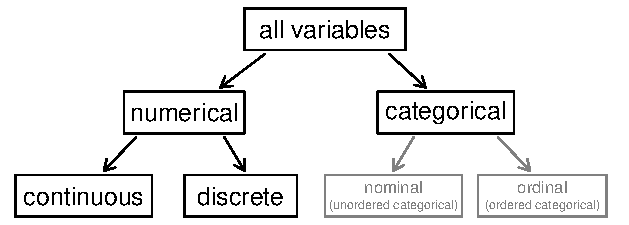
\includegraphics[width=0.57\textwidth]{ch_intro_to_data/figures/variables/variables}
\caption{Breakdown of variables into their respective types.}
\label{variables}
\end{figure}

Finally, consider the \var{smoking\_\hspace{0.3mm}ban} variable, which describes the type of county-wide smoking ban and takes values \resp{none}, \resp{partial}, or \resp{comprehensive} in each county. This variable seems to be a hybrid: it is a categorical variable but the levels have a natural ordering. A variable with these properties is called an \term{ordinal} variable, while a regular categorical variable without this type of special ordering is called a \term{nominal} variable. To simplify analyses, any ordinal variables in this book will be treated as categorical variables.

\begin{example}{Data were collected about students in a statistics course. Three variables were recorded for each student: number of siblings, student height, and whether the student had previously taken a statistics course. Classify each of the variables as continuous numerical, discrete numerical, or categorical.}
The number of siblings and student height represent numerical variables. Because the number of siblings is a count, it is discrete. Height varies continuously, so it is a continuous numerical variable. The last variable classifies students into two categories -- those who have and those who have not taken a statistics course -- which makes this variable categorical.
\end{example}

\begin{exercise} \index{data!stroke}
Consider the variables \var{group} and \var{outcome} (at 30 days) from the stent study in Section~\ref{basicExampleOfStentsAndStrokes}. Are these numerical or categorical variables?\footnote{There are only two possible values for each variable, and in both cases they describe categories. Thus, each is categorical variables.}
\end{exercise}

\subsection{Relationships between variables}
\label{variableRelations}

Many analyses are motivated by a researcher looking for a relationship between two or more variables. A social scientist may like to answer some of the following questions:
\begin{enumerate}
\setlength{\itemsep}{0mm}
\item[(1)]\label{fedSpendingPovertyQuestion} Is federal spending, on average, higher or lower in counties with high rates of poverty?
\item[(2)]\label{ownershipMultiUnitQuestion} If homeownership is lower than the national average in one county, will the percent of multi-unit structures in that county likely be above or below the national average?
\item[(3)]\label{isAverageIncomeAssociatedWithSmokingBans} Which counties have a higher average income: those that enact one or more smoking bans or those that do not?
\end{enumerate}

To answer these questions, data must be collected, such as the \data{county} data set shown in Table~\ref{countyDF}. Examining summary statistics \index{summary statistic} could provide insights for each of the three questions about counties. Additionally, graphs can be used to visually summarize data and are useful for answering such questions as well.

\indexthis{Scatterplots}{scatterplot} are one type of graph used to study the relationship between two numerical variables. Figure~\ref{county_fed_spendVsPoverty} compares the variables \var{fed\_\hspace{0.3mm}spend} and \var{poverty}. Each point on the plot represents a single county. For instance, the highlighted dot corresponds to County~1088 in the \data{county} data set: Owsley County, Kentucky, which had a poverty rate of 41.5\% and federal spending of \$21.50 per capita. The scatterplot suggests a relationship between the two variables: counties with a high poverty rate also tend to have slightly more federal spending. We might brainstorm as to why this relationship exists and investigate each idea to determine which is the most reasonable explanation.

\begin{figure}
\centering
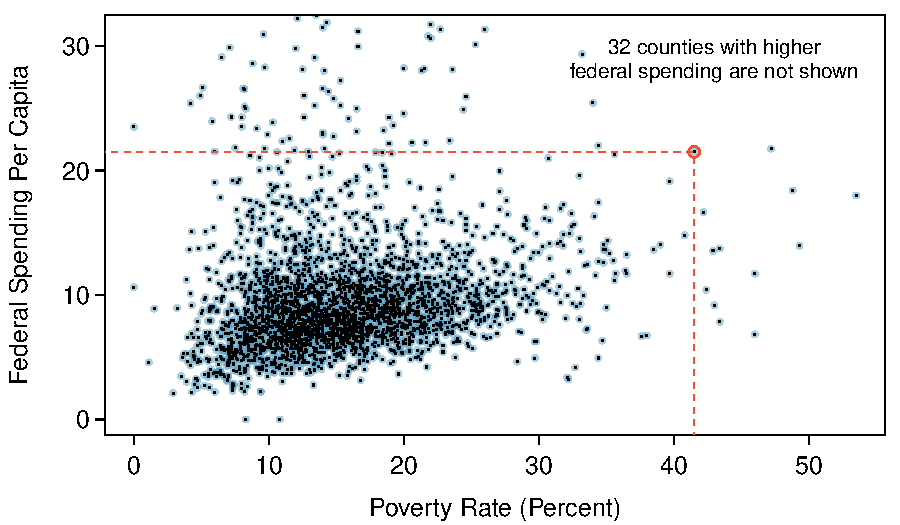
\includegraphics[width=0.8\textwidth]{ch_intro_to_data/figures/county_fed_spendVsPoverty/county_fed_spendVsPoverty}
\caption{A scatterplot showing \var{fed\_\hspace{0.3mm}spend} against \var{poverty}. Owsley County of Kentucky, with a poverty rate of 41.5\% and federal spending of \$21.50 per capita, is highlighted.}
\label{county_fed_spendVsPoverty}
\end{figure}

\begin{exercise}
Examine the variables in the \data{email50} data set, which are described in Table~\vref{email50Variables}. Create two questions about the relationships between these variables that are of interest to you.\footnote{Two sample questions: (1) Intuition suggests that if there are many line breaks in an email then there also would tend to be many characters: does this hold true? (2)~Is there a connection between whether an email format is plain text (versus HTML) and whether it is a spam message?}
\end{exercise}

The \var{fed\_\hspace{0.3mm}spend} and \var{poverty} variables are said to be associated because the plot shows a discernible pattern. When two variables show some connection with one another, they are called \term{associated} variables. Associated variables can also be called \term{dependent} variables and vice-versa.

\begin{example}{This example examines the relationship between homeownership and the percent of units in multi-unit structures (e.g. apartments, condos), which is visualized using a scatterplot in Figure~\ref{multiunitsVsOwnership}. Are these variables associated?}
It appears that the larger the fraction of units in multi-unit structures, the lower the homeownership rate. Since there is some relationship between the variables, they are associated.
\end{example}


\begin{figure}
   \centering
   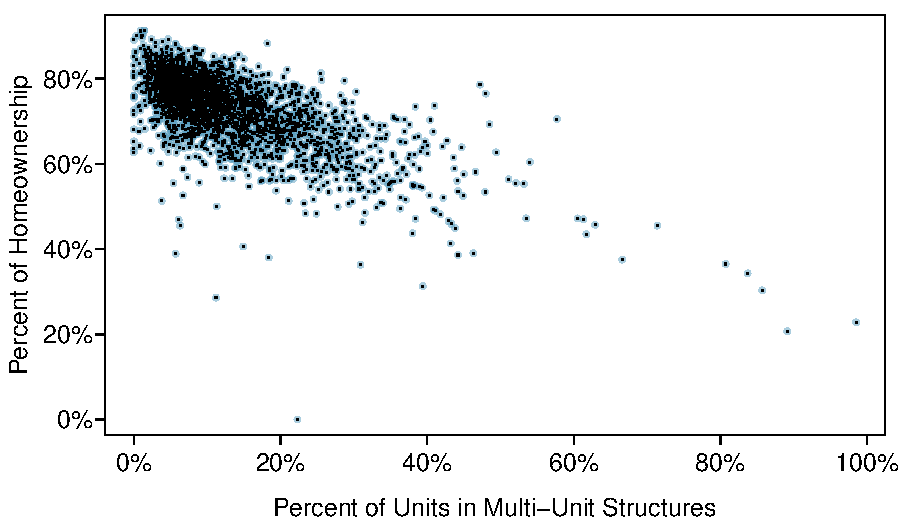
\includegraphics[width=0.8\textwidth]{ch_intro_to_data/figures/multiunitsVsOwnership/multiunitsVsOwnership}
   \caption{A scatterplot of homeownership versus the percent of units that are in multi-unit structures for all 3,143 counties. Interested readers may find an image of this plot with an additional third variable, county population, presented at \oiRedirect{textbook-homeownership_vs_multi_unit_structures}{www.openintro.org/stat/down/MHP.png}.}
   \label{multiunitsVsOwnership}
\end{figure}

Because there is a downward trend in Figure~\ref{multiunitsVsOwnership} -- counties with more units in multi-unit structures are associated with lower homeownership -- these variables are said to be \termsub{negatively associated}{negative association}. A \term{positive association} is shown in the relationship between the \var{poverty} and \var{fed\_\hspace{0.3mm}spend} variables represented in Figure~\ref{county_fed_spendVsPoverty}, where counties with higher poverty rates tend to receive more federal spending per capita.

If two variables are not associated, then they are said to be \term{independent}. That is, two variables are independent if there is no evident relationship between the two.

\begin{termBox}{\tBoxTitle{Associated or independent, not both}
A pair of variables are either related in some way (associated) or not (independent). No pair of variables is both associated and independent.}
\end{termBox}

\index{data!county|)}

%%%%%
\section[Overview of data collection principles]{Overview of data collection principles \sectionvideohref{youtube-2N_bkiyTiXU&list=PLkIselvEzpM6pZ76FD3NoCvvgkj_p-dE8}}
\label{overviewOfDataCollectionPrinciples}

\index{sample|(}
\index{population|(}

The first step in conducting research is to identify topics or questions that are to be investigated. A clearly laid out research question is helpful in identifying what subjects or cases should be studied and what variables are important. It is also important to consider \emph{how} data are collected so that they are reliable and help achieve the research goals.

\subsection{Populations and samples}
\label{populationsAndSamples}

Consider the following three research questions:
\begin{enumerate}
\setlength{\itemsep}{0mm}
\item What is the average mercury content in swordfish in the Atlantic Ocean?
\item\label{timeToGraduationQuestionForUCLAStudents} Over the last 5 years, what is the average time to complete a degree for Duke undergraduate students?
\item\label{identifyPopulationOfStentStudy} Does a new drug reduce the number of deaths in patients with severe heart disease?
\end{enumerate}
Each research question refers to a target \term{population}. In the first question, the target population is all swordfish in the Atlantic ocean, and each fish represents a case. Often times, it is too expensive to collect data for every case in a population. Instead, a sample is taken. A \term{sample} represents a subset of the cases and is often a small fraction of the population. For instance, 60 swordfish (or some other number) in the population might be selected, and this sample data may be used to provide an estimate of the population average and answer the research question.

\begin{exercise} \label{identifyingThePopulationForTwoQuestionsInPopAndSampSubsection}
For the second and third questions above, identify the target population and what represents an individual case.\footnote{(\ref{timeToGraduationQuestionForUCLAStudents}) Notice that the first question is only relevant to students who complete their degree; the average cannot be computed using a student who never finished her degree. Thus, only Duke undergraduate students who have graduated in the last five years represent cases in the population under consideration. Each such student would represent an individual case. (\ref{identifyPopulationOfStentStudy}) A person with severe heart disease represents a case. The population includes all people with severe heart disease.}
\end{exercise}


\subsection{Anecdotal evidence}
\label{anecdotalEvidenceSubsection}

Consider the following possible responses to the three research questions:
\begin{enumerate}
\item A man on the news got mercury poisoning from eating swordfish, so the average mercury concentration in swordfish must be dangerously high.
\item\label{iKnowThreeStudentsWhoTookMoreThan7YearsToGraduateAtDuke} I met two students who took more than 7 years to graduate from Duke, so it must take longer to graduate at Duke than at many other colleges.
\item\label{myFriendsDadDiedAfterSulphinpyrazon} My friend's dad had a heart attack and died after they gave him a new heart disease drug, so the drug must not work.
\end{enumerate}
Each conclusion is based on data. However, there are two problems. First, the data only represent one or two cases. Second, and more importantly, it is unclear whether these cases are actually representative of the population. Data collected in this haphazard fashion are called \term{anecdotal evidence}.

\setlength{\captionwidth}{\textwidth-80mm}
\begin{figure}
\centering
\hspace{8mm}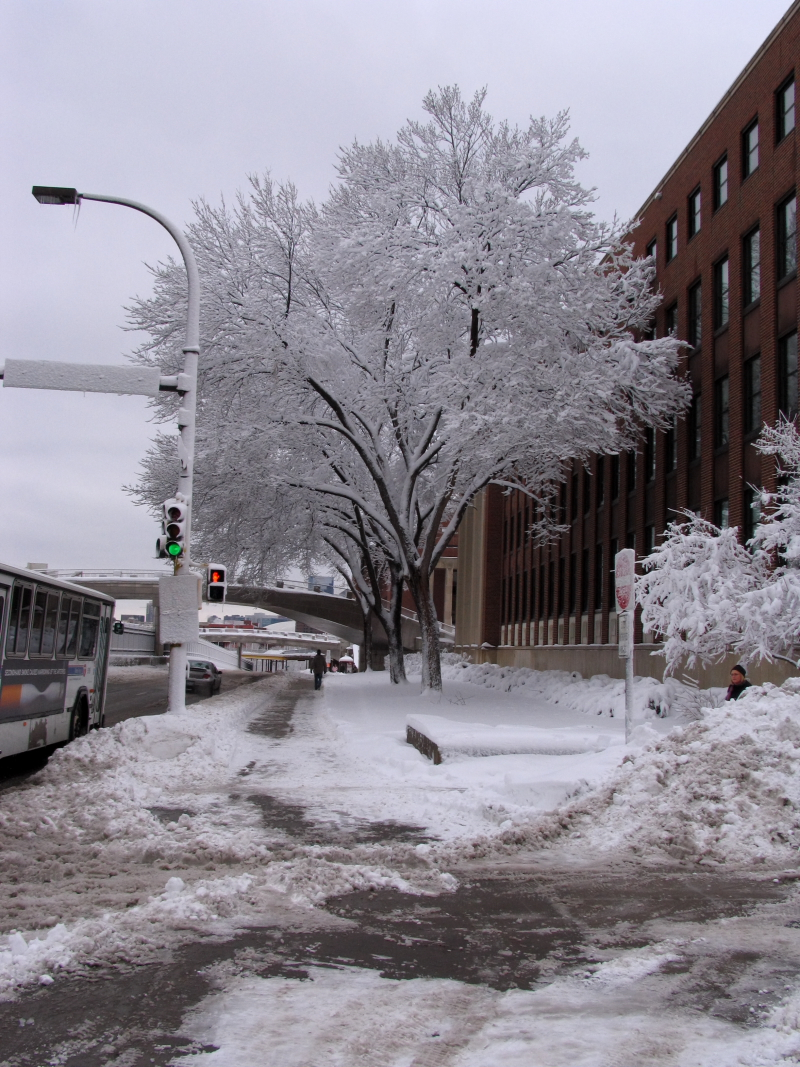
\includegraphics[width=55mm]{ch_intro_to_data/figures/mnWinter/mnWinter}\hspace{4mm}
\begin{minipage}[b]{\textwidth - 80mm}
   \caption[anecdotal evidence]{In February 2010, some media pundits cited one large snow storm as valid evidence against global warming. As comedian Jon Stewart pointed out, ``It's one storm, in one region, of one country.''
   \label{mnWinter}}
\end{minipage}
\end{figure}
\setlength{\captionwidth}{\mycaptionwidth}

\begin{termBox}{\tBoxTitle{Anecdotal evidence}
Be careful of data collected in a haphazard fashion. Such evidence may be true and verifiable, but it may only represent extraordinary cases.}
\end{termBox}

Anecdotal evidence typically is composed of unusual cases that we recall based on their striking characteristics. For instance, we are more likely to remember the two people we met who took 7 years to graduate than the six others who graduated in four years. Instead of looking at the most unusual cases, we should examine a sample of many cases that represent the population.

\subsection{Sampling from a population}

\index{sample!random sample|(}

We might try to estimate the time to graduation for Duke undergraduates in the last 5 years by collecting a sample of students. All graduates in the last 5 years represent the \emph{population}\index{population}, and graduates who are selected for review are collectively called the \emph{sample}\index{sample}. In general, we always seek to \emph{randomly} select a sample from a population. The most basic type of random selection is equivalent to how raffles are conducted. For example, in selecting graduates, we could write each graduate's name on a raffle ticket and draw 100 tickets. The selected names would represent a random sample of 100 graduates.

\begin{figure}[ht]
\centering
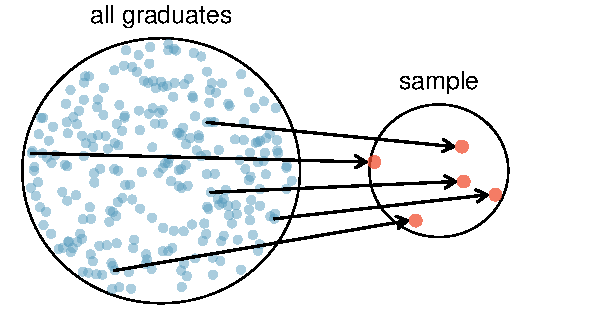
\includegraphics[width=0.47\textwidth]{ch_intro_to_data/figures/popToSample/popToSampleGraduates}
\caption{In this graphic, five graduates are randomly selected from the population to be included in the sample.}
\label{popToSampleGraduates}
\end{figure}

Why pick a sample randomly? Why not just pick a sample by hand? Consider the following scenario.

\begin{example}{Suppose we ask a student who happens to be majoring in nutrition to select several graduates for the study. What kind of students do you think she might collect? Do you think her sample would be representative of all graduates?}
Perhaps she would pick a disproportionate number of graduates from health-related fields. Or perhaps her selection would be well-representative of the population. When selecting samples by hand, we run the risk of picking a \emph{biased} sample, even if that bias is unintentional or difficult to discern.
\end{example}

\begin{figure}
\centering
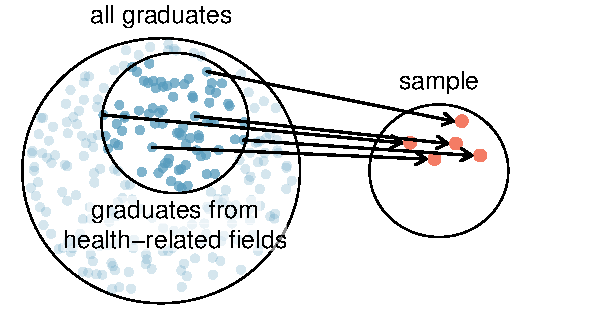
\includegraphics[width=0.47\textwidth]{ch_intro_to_data/figures/popToSample/popToSubSampleGraduates}
\caption{Instead of sampling from all graduates equally, a nutrition major might inadvertently pick graduates with health-related majors disproportionately often.}
\label{popToSubSampleGraduates}
\end{figure}

If someone was permitted to pick and choose exactly which graduates were included in the sample, it is entirely possible that the sample could be skewed to that person's interests, which may be entirely unintentional. This introduces \term{bias} into a sample. Sampling randomly helps resolve this problem. The most basic random sample is called a \term{simple random sample}, and which is equivalent to using a raffle to select cases. This means that each case in the population has an equal chance of being included and there is no implied connection between the cases in the sample.

\APVersion{Sometimes a simple random sample is difficult to implement and an alternative method is helpful. One such substitute is a \term{systematic sample}, where one case is sampled after letting a fixed number of others, say 10 other cases, pass by. Since this approach uses a mechanism that is not easily subject to personal biases, it often yields a reasonably representative sample. This book will focus on random samples since the use of systematic samples is uncommon and requires additional considerations of the context.}{}

The act of taking a simple random sample helps minimize bias, however, bias can crop up in other ways.
Even when people are picked at random, e.g. for surveys, caution must be exercised if the \term{non-response} \index{sample!non-response|textbf} is high. For instance, if only 30\% of the people randomly sampled for a survey actually respond, then it is unclear whether the results are \term{representative} of the entire population. This \term{non-response bias} \index{sample!non-response bias|textbf} can skew results.

\begin{figure}[h]
\centering
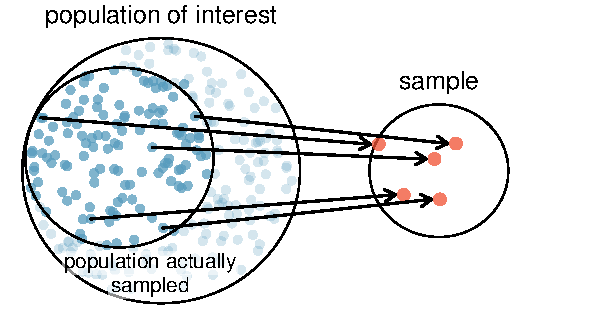
\includegraphics[width=0.5\textwidth]{ch_intro_to_data/figures/popToSample/surveySample}
\caption{Due to the possibility of non-response, surveys studies may only reach a certain group within the population. It is difficult, and often times impossible, to completely fix this problem.}
\label{surveySample}
\end{figure}

Another common downfall is a \term{convenience sample}\index{sample!convenience sample}, where individuals who are easily accessible are more likely to be included in the sample. For instance, if a political survey is done by stopping people walking in the Bronx, this will not represent all of New York City. It is often difficult to discern what sub-population a convenience sample represents.

\begin{exercise}
We can easily access ratings for products, sellers, and companies through websites. These ratings are based only on those people who go out of their way to provide a rating. If 50\% of online reviews for a product are negative, do you think this means that 50\% of buyers are dissatisfied with the product?\footnote{Answers will vary. From our own anecdotal experiences, we believe people tend to rant more about products that fell below expectations than rave about those that perform as expected. For this reason, we suspect there is a negative bias in product ratings on sites like Amazon. However, since our experiences may not be representative, we also keep an open mind.}
\end{exercise}

\index{sample!random sample|)}
\index{population|)}
\index{sample|)}

\subsection{Explanatory and response variables}
\label{explanatoryAndResponse}

\index{data!county|(}

Consider the following question from page~\pageref{fedSpendingPovertyQuestion} for the \data{county} data set:
\begin{enumerate}
\item[(1)] 
	Is federal spending, on average, higher or lower in counties with high rates of poverty?
\end{enumerate}
If we suspect poverty might affect spending in a county, then poverty is the \term{explanatory} variable and federal spending is the \term{response} variable in the relationship.\footnote{Sometimes the explanatory variable is called the \term{independent} variable and the response variable is called the \term{dependent} variable. However, this becomes confusing since a \emph{pair} of variables might be independent or dependent, so we avoid this language.} If there are many variables, it may be possible to consider a number of them as explanatory variables.

\begin{tipBox}{\tipBoxTitle{Explanatory and response variables}
To identify the explanatory variable in a pair of variables, identify which of the two is suspected of affecting the other and plan an appropriate analysis.

\hspace{10mm}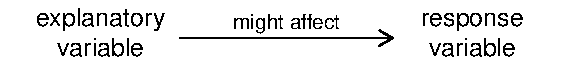
\includegraphics[height=0.34in]{ch_intro_to_data/figures/expResp/expResp}}
\end{tipBox}

\begin{caution}{association does not imply causation}{Labeling variables as \emph{explanatory} and \emph{response} does not guarantee the relationship between the two is actually causal, even if there is an association identified between the two variables. We use these labels only to keep track of which variable we suspect affects the other.}
\end{caution}

In some cases, there is no explanatory or response variable. Consider the following question from page~\pageref{ownershipMultiUnitQuestion}:
\begin{enumerate}
\item[(2)] 
	If homeownership is lower than the national average in one county, will the percent of multi-unit structures in that county likely be above or below the national average?
\end{enumerate}
It is difficult to decide which of these variables should be considered the explanatory and response variable, i.e. the direction is ambiguous, so no explanatory or response labels are suggested here.

\index{data!county|)}

\subsection{Introducing observational studies and experiments}

There are two primary types of data collection: observational studies and experiments.

Researchers perform an \term{observational study} when they collect data in a way that does not directly interfere with how the data arise. For instance, researchers may collect information via surveys, review medical or company records, or follow a \term{cohort} of many similar individuals to study why certain diseases might develop. In each of these situations, researchers merely observe the data that arise. In general, observational studies can provide evidence of a naturally occurring association between variables, but they cannot by themselves show a causal connection.

When researchers want to investigate the possibility of a causal connection, they conduct an \term{experiment}. Usually there will be both an explanatory and a response variable. For instance, we may suspect administering a drug will reduce mortality in heart attack patients over the following year. To check if there really is a causal connection between the explanatory variable and the response, researchers will collect a sample of individuals and split them into groups. The individuals in each group are \emph{assigned} a treatment. When individuals are randomly assigned to a group, the experiment is called a \term{randomized experiment}. For example, each heart attack patient in the drug trial could be randomly assigned,  perhaps by flipping a coin, into one of two groups: the first group receives a \term{placebo} (fake treatment) and the second group receives the drug. See the case study in Section~\ref{basicExampleOfStentsAndStrokes} for another example of an experiment, though that study did not employ a placebo.

\begin{tipBox}{\tipBoxTitle{association $\neq$ causation}
In general, association does not imply causation, and causation can only be inferred from a randomized experiment.}
\end{tipBox}


%%%%%
\section[Observational studies and sampling strategies]{Observational studies and sampling strategies \sectionvideohref{youtube-n1xSeGPGQEg&list=PLkIselvEzpM6pZ76FD3NoCvvgkj_p-dE8}}

\subsection{Observational studies}

Generally, data in observational studies are collected only by monitoring what occurs, while experiments require the primary explanatory variable in a study be assigned for each subject by the researchers.

Making causal conclusions based on experiments is often reasonable. However, making the same causal conclusions based on observational data can be treacherous and is not recommended. Thus, observational studies are generally only sufficient to show associations.

\begin{exercise} \label{sunscreenLurkingExample}
Suppose an observational study tracked sunscreen use and skin cancer, and it was found that the more sunscreen someone used, the more likely the person was to have skin cancer. Does this mean sunscreen \emph{causes} skin cancer?\footnote{No. See the paragraph following the exercise for an explanation.}
\end{exercise}

Some previous research tells us that using sunscreen actually reduces skin cancer risk, so maybe there is another variable that can explain this hypothetical association between sunscreen usage and skin cancer. One important piece of information that is absent is sun exposure. If someone is out in the sun all day, she is more likely to use sunscreen \emph{and} more likely to get skin cancer. Exposure to the sun is unaccounted for in the simple investigation.
\begin{center}
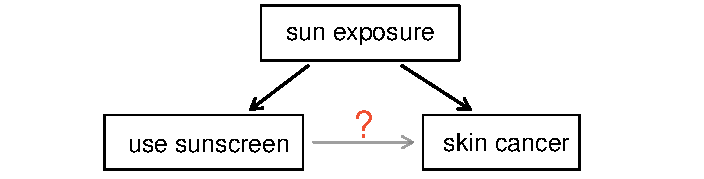
\includegraphics[height=1.0in]{ch_intro_to_data/figures/variables/sunCausesCancer}
\end{center}
% Some studies:
% http://www.sciencedirect.com/science/article/pii/S0140673698121682
% http://archderm.ama-assn.org/cgi/content/abstract/122/5/537
% Study with a similar scenario to that described here:
% http://onlinelibrary.wiley.com/doi/10.1002/ijc.22745/full

Sun exposure is what is called a \term{confounding variable},\footnote{Also called a \term{lurking variable}, \term{confounding factor}, or a \term{confounder}.} which is a variable that is correlated with both the explanatory and response variables. While one method to justify making causal conclusions from observational studies is to exhaust the search for confounding variables, there is no guarantee that all confounding variables can be examined or measured.

In the same way, the \data{county} data set is an observational study with confounding variables, and its data cannot easily be used to make causal conclusions.

\begin{exercise}
Figure~\ref{multiunitsVsOwnership} shows a negative association between the homeownership rate and the percentage of multi-unit structures in a county. However, it is unreasonable to conclude that there is a causal relationship between the two variables. Suggest one or more other variables that might explain the relationship visible in Figure~\ref{multiunitsVsOwnership}.\footnote{Answers will vary. Population density may be important. If a county is very dense, then this may require a larger fraction of residents to live in multi-unit structures. Additionally, the high density may contribute to increases in property value, making homeownership infeasible for many residents.}
\end{exercise}

Observational studies come in two forms: prospective and retrospective studies. A \term{prospective study} identifies individuals and collects information as events unfold. For instance, medical researchers may identify and follow a group of similar individuals over many years to assess the possible influences of behavior on cancer risk. One example of such a study is The Nurses' Health Study, started in 1976 and expanded in 1989.\footnote{\oiRedirect{textbook-channing_nurse_study}{www.channing.harvard.edu/nhs}} This prospective study recruits registered nurses and then collects data from them using questionnaires. \termsub{Retrospective studies}{retrospective studies} collect data after events have taken place, e.g. researchers may review past events in medical records. Some data sets, such as \data{county}, may contain both prospectively- and retrospectively-collected variables. Local governments prospectively collect some variables as events unfolded (e.g. retails sales) while the federal government retrospectively collected others during the 2010 census (e.g. county population counts).

\subsection{Four sampling methods (special topic)}
\label{fourSamplingMethods}
\label{threeSamplingMethods}

Almost all statistical methods are based on the notion of implied randomness. If observational data are not collected in a random framework from a population, these statistical methods -- the estimates and errors associated with the estimates -- are not reliable. Here we consider four random sampling techniques: simple, stratified, cluster, and multistage sampling. Figures~\ref{simple_stratified} and~\ref{cluster_multistage} provide graphical representations of these techniques.

\begin{figure}
\centering
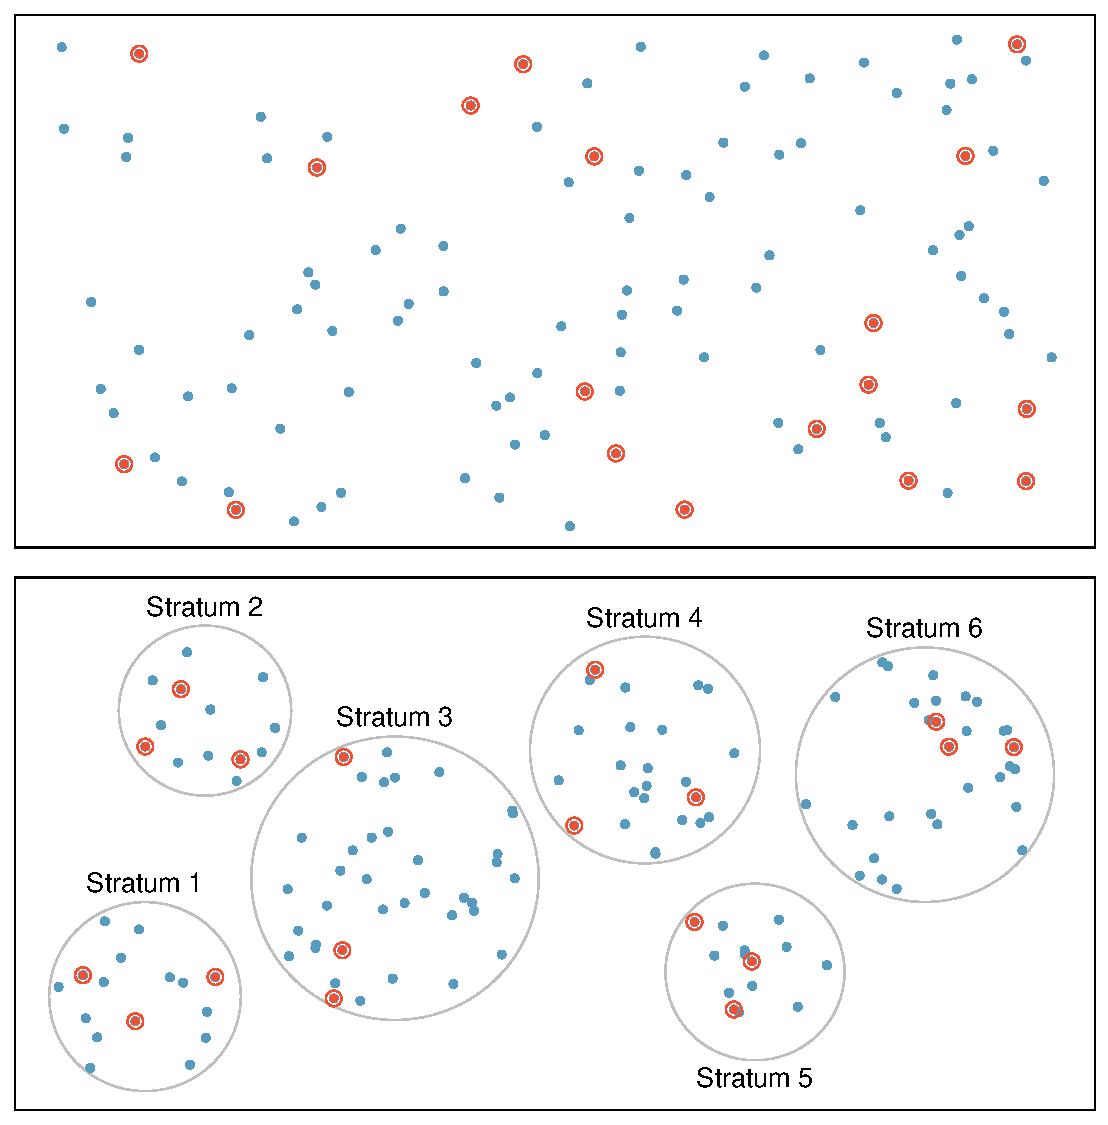
\includegraphics[width=\textwidth]{ch_intro_to_data/figures/samplingMethodsFigure/simple_stratified}
\caption{Examples of simple random\index{sample!simple random sampling} and stratified sampling\index{sample!stratified sampling}. In the top panel, simple random sampling was used to randomly select the 18 cases. In the bottom panel, stratified sampling was used: cases were grouped into strata, then simple random sampling was employed within \mbox{each stratum}.}
\label{simple_stratified}
\end{figure}

\termsub{Simple random sampling}{sample!simple random sampling} is probably the most intuitive form of random sampling. Consider the salaries of Major League Baseball (MLB) players, where each player is a member of one of the league's 30 teams. To take a simple random sample of 120 baseball players and their salaries from the 2010 season, we could write the names of that season's 828 players onto slips of paper, drop the slips into a bucket, shake the bucket around until we are sure the names are all mixed up, then draw out slips until we have the sample of 120 players. In general, a sample is referred to as ``simple random'' if each case in the population has an equal chance of being included in the final sample \emph{and} knowing that a case is included in a sample does not provide useful information about which other cases are included.

\termsub{Stratified sampling}{sample!stratified sampling} is a divide-and-conquer sampling strategy. The population is divided into groups called \term{strata}\index{sample!strata|textbf}. The strata are chosen so that similar cases are grouped together, then a second sampling method, usually simple random sampling, is employed within each stratum. In the baseball salary example, the teams could represent the strata, since some teams have a lot more money (up to 4~times as much!). Then we might randomly sample 4 players from each team for a total of 120 players.

Stratified sampling is especially useful when the cases in each stratum are very similar with respect to the outcome of interest. The downside is that analyzing data from a stratified sample is a more complex task than analyzing data from a simple random sample. The analysis methods introduced in this book would need to be extended to analyze data collected using stratified sampling.

\begin{example}{Why would it be good for cases within each stratum to be very similar?}
We might get a more stable estimate for the subpopulation in a stratum if the cases are very similar. These improved estimates for each subpopulation will help us build a reliable estimate for the full population.
\end{example}

In a \termsub{cluster sample}{sample!cluster sample}, we break up the population into many groups, called \termsub{clusters}{sample!cluster}. Then we sample a fixed number of clusters and include all observations from each of those clusters in the sample. A \termsub{multistage sample}{sample!multistage sample} is like a cluster sample, but rather than keeping all observations in each cluster, we collect a random sample within each selected cluster. %Multistage sampling is similar to stratified sampling in its process, except that stratified sampling requires observations be sampled from \emph{every} stratum.

\begin{figure}
\centering
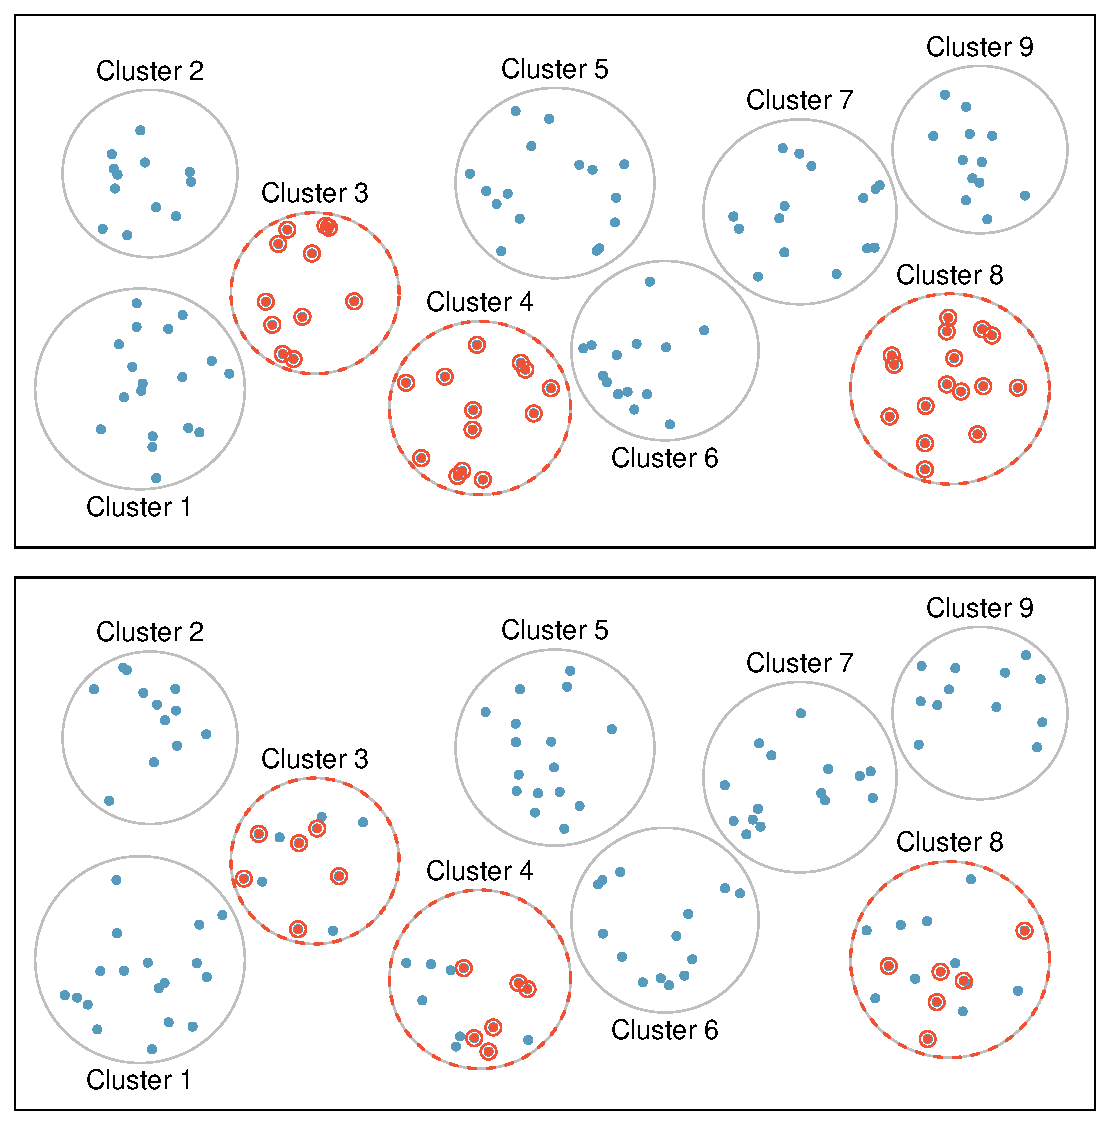
\includegraphics[width=\textwidth]{ch_intro_to_data/figures/samplingMethodsFigure/cluster_multistage}
\caption{Examples of cluster\index{sample!cluster sampling} and multistage sampling\index{sample!multistage sampling}. In the top panel, cluster sampling was used. Here, data were binned into nine clusters, three of these clusters were sampled, and all observations within these three cluster were included in the sample. In the bottom panel, multistage sampling was used.
It differs from cluster sampling in that of the clusters selected, we randomly select a subset of each cluster to be included in the sample.}
\label{cluster_multistage}
\end{figure}

Sometimes cluster or multistage sampling can be more economical than the alternative sampling techniques. Also, unlike stratified sampling, these approaches are most helpful when there is a lot of case-to-case variability within a cluster but the clusters themselves don't look very different from one another. For example, if neighborhoods represented clusters, then cluster or multistage sampling work best when the neighborhoods are very diverse. A downside of these methods is that more advanced analysis techniques are typically required, though the methods in this book can be extended to handle such data.

\begin{example}{Suppose we are interested in estimating the malaria rate in a densely tropical portion of rural Indonesia. We learn that there are 30 villages in that part of the Indonesian jungle, each more or less similar to the next. Our goal is to test 150 individuals for malaria. What sampling method should be employed?}
A simple random sample would likely draw individuals from all 30 villages, which could make data collection extremely expensive. Stratified sampling would be a challenge since it is unclear how we would build strata of similar individuals. However, cluster sampling or multistage sampling seem like very good ideas. If we decided to use multistage sampling, we might randomly select half of the villages, then randomly select 10 people from each. This would probably reduce our data collection costs substantially in comparison to a simple random sample, and this approach would still give us reliable information.
\end{example}


%%%%%
\section[Experiments]{Experiments \sectionvideohref{youtube-g7JGe_ykB3I&list=PLkIselvEzpM6pZ76FD3NoCvvgkj_p-dE8}}
\label{experimentsSection}

Studies where the researchers assign treatments to cases are called \termsub{experiments}{experiment}. When this assignment includes randomization, e.g.~using a coin flip to decide which treatment a patient receives, it is called a \term{randomized experiment}. Randomized experiments are fundamentally important when trying to show a causal connection between two variables.

\subsection{Principles of experimental design}
\label{experimentalDesignPrinciples}

Randomized experiments are generally built on four principles.
\begin{description}
\item[Controlling.] Researchers assign treatments to cases, and they do their best to \term{control} any other differences in the groups. For example, when patients take a drug in pill form, some patients take the pill with only a sip of water while others may have it with an entire glass of water. To control for the effect of water consumption, a doctor may ask all patients to drink a 12 ounce glass of water with the pill.
\item[Randomization.] Researchers randomize patients into treatment groups to account for variables that cannot be controlled. For example, some patients may be more susceptible to a disease than others due to their dietary habits. Randomizing patients into the treatment or control group helps even out such differences, and it also prevents accidental bias from entering the study.
\item[Replication.] The more cases researchers observe, the more accurately they can estimate the effect of the explanatory variable on the response. In a single study, we \term{replicate} by collecting a sufficiently large sample. Additionally, a group of scientists may replicate an entire study to verify an earlier finding.

\begin{figure}
\centering
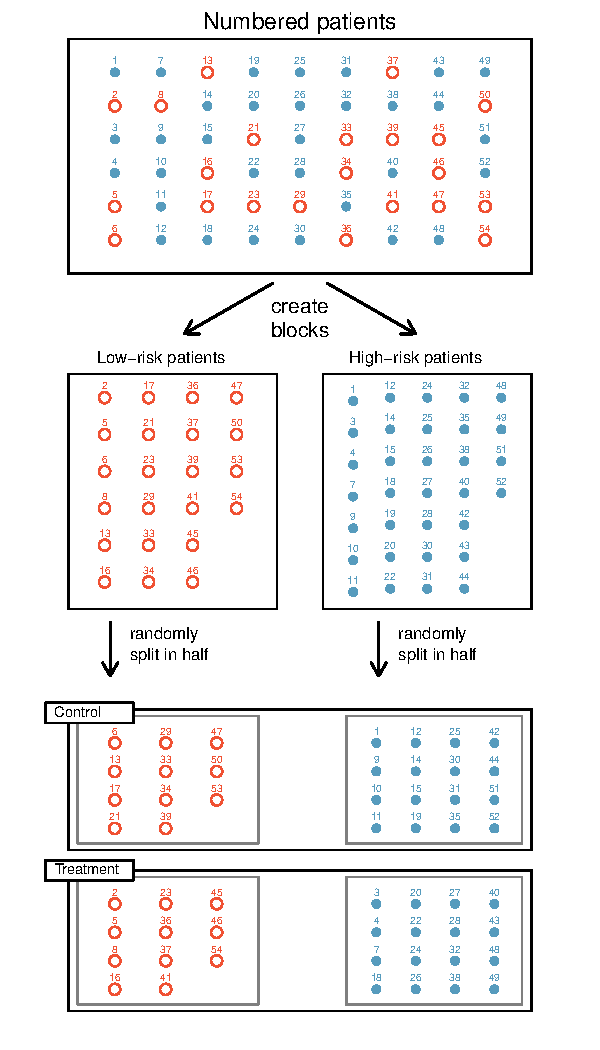
\includegraphics[width=0.78\textwidth]{ch_intro_to_data/figures/figureShowingBlocking/figureShowingBlocking}
\caption{Blocking using a variable depicting patient risk. Patients are first divided into low-risk and high-risk blocks, then each block is evenly separated into the treatment groups using randomization. This strategy ensures an equal representation of patients in each treatment group from both the low-risk and high-risk categories.}
\label{figureShowingBlocking}
\end{figure}

\item[Blocking.] Researchers sometimes know or suspect that variables, other than the treatment, influence the response. Under these circumstances, they may first group individuals based on this variable into \term{blocks} and then randomize cases within each block to the treatment groups. This strategy is often referred to as \term{blocking}. For instance, if we are looking at the effect of a drug on heart attacks, we might first split patients in the study into low-risk and high-risk blocks, then randomly assign half the patients from each block to the control group and the other half to the treatment group, as shown in Figure~\ref{figureShowingBlocking}. This strategy ensures each treatment group has an equal number of low-risk and high-risk patients.
\end{description}

It is important to incorporate the first three experimental design principles into any study, and this book describes applicable methods for analyzing data from such experiments. Blocking is a slightly more advanced technique, and statistical methods in this book may be extended to analyze data collected using blocking.

\subsection{Reducing bias in human experiments}
\label{biasInHumanExperiments}

Randomized experiments are the gold standard for data collection, but they do not ensure an unbiased perspective into the cause and effect relationships in all cases. Human studies are perfect examples where bias can unintentionally arise. Here we reconsider a study where a new drug was used to treat heart attack patients.\footnote{Anturane Reinfarction Trial Research Group. 1980. Sulfinpyrazone in the prevention of sudden death after myocardial infarction. New England Journal of Medicine 302(5):250-256.} In particular, researchers wanted to know if the drug reduced deaths in patients.

These researchers designed a randomized experiment because they wanted to draw causal conclusions about the drug's effect. Study volunteers\footnote{Human subjects are often called \term{patients}, \term{volunteers}, or \term{study participants}.} were randomly placed into two study groups. One group, the \term{treatment group}, received the drug. The other group, called the \term{control group}, did not receive any drug treatment.

Put yourself in the place of a person in the study. If you are in the treatment group, you are given a fancy new drug that you anticipate will help you. On the other hand, a person in the other group doesn't receive the drug and sits idly, hoping her participation doesn't increase her risk of death. These perspectives suggest there are actually two effects: the one of interest is the effectiveness of the drug, and the second is an emotional effect that is difficult to quantify.

Researchers aren't usually interested in the emotional effect, which might bias the study. To circumvent this problem, researchers do not want patients to know which group they are in. When researchers keep the patients uninformed about their treatment, the study is said to be \term{blind}. But there is one problem: if a patient doesn't receive a treatment, she will know she is in the control group. The solution to this problem is to give fake treatments to patients in the control group. A fake treatment is called a \term{placebo}, and an effective placebo is the key to making a study truly blind. A classic example of a placebo is a sugar pill that is made to look like the actual treatment pill. Often times, a placebo results in a slight but real improvement in patients. This effect has been dubbed the \term{placebo~effect}.

The patients are not the only ones who should be blinded: doctors and researchers can accidentally bias a study. When a doctor knows a patient has been given the real treatment, she might inadvertently give that patient more attention or care than a patient that she knows is on the placebo. To guard against this bias, which again has been found to have a measurable effect in some instances, most modern studies employ a \term{double-blind} setup where doctors or researchers who interact with patients are, just like the patients, unaware of who is or is not receiving the treatment.\footnote{There are always some researchers involved in the study who do know which patients are receiving which treatment. However, they do not interact with the study's patients and do not tell the blinded health care professionals who is receiving which treatment.}

\begin{exercise}
Look back to the study in Section~\ref{basicExampleOfStentsAndStrokes} where researchers were testing whether stents were effective at reducing strokes in at-risk patients. Is this an experiment? Was the study blinded? Was it double-blinded?\footnote{The researchers assigned the patients into their treatment groups, so this study was an experiment. However, the patients could distinguish what treatment they received, so this study was not blind. The study could not be double-blind since it was not blind.}
\end{exercise}


%%%%%
\section[Examining numerical data]{Examining numerical data \sectionvideohref{youtube-Xm0PPtci3JE&list=PLkIselvEzpM6pZ76FD3NoCvvgkj_p-dE8}}
\label{numericalData}

In this section we will be introduced to techniques for exploring and summarizing numerical variables. The \data{email50} and \data{county} data sets from Section~\ref{dataBasics} provide rich opportunities for examples. Recall that outcomes of numerical variables are numbers on which it is reasonable to perform basic arithmetic operations. For example, the \var{pop2010} variable, which represents the populations of counties in 2010, is numerical since we can sensibly discuss the difference or ratio of the populations in two counties. On the other hand, area codes and zip codes are not numerical, but rather they are~categorical variables.


\subsection{Scatterplots for paired data}
\label{scatterPlots}

\index{data!email50|(}

A \term{scatterplot} provides a case-by-case view of data for two numerical variables. In Figure~\vref{county_fed_spendVsPoverty}, a scatterplot was used to examine how federal spending and poverty were related in the \data{county} data set. Another scatterplot is shown in Figure~\ref{email50LinesCharacters}, comparing the number of line breaks (\var{line\_\hspace{0.3mm}breaks}) and number of characters (\var{num\_\hspace{0.3mm}char}) in emails for the \data{email50} data set. In any scatterplot, each point represents a single case. Since there are 50 cases in \data{email50}, there are 50 points in Figure~\ref{email50LinesCharacters}.

\textC{\setlength{\captionwidth}{0.9\textwidth}}

\begin{figure}[h]
   \centering
   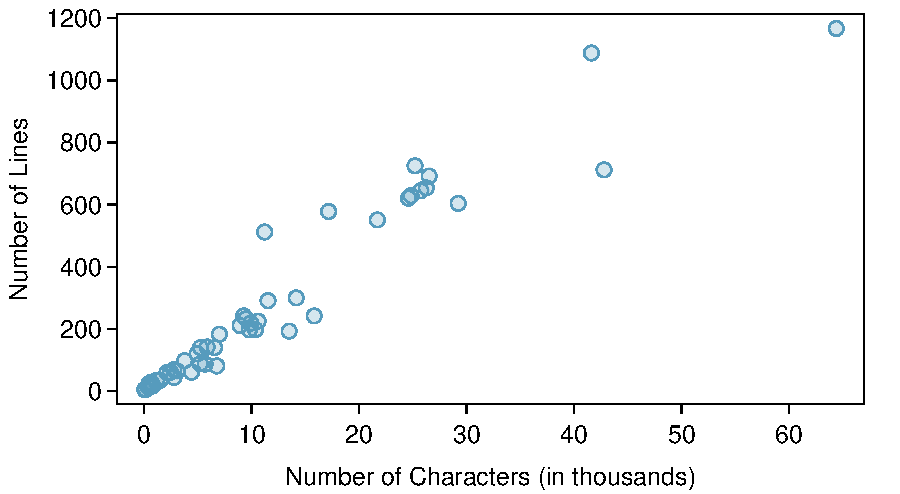
\includegraphics[width=0.8\textwidth]{ch_intro_to_data/figures/email50LinesCharacters/email50LinesCharacters}
   \caption{A scatterplot of \var{line\_\hspace{0.3mm}breaks} versus \var{num\_\hspace{0.3mm}char} for the \data{email50} data.}
   \label{email50LinesCharacters}
\end{figure}

\textC{\setlength{\captionwidth}{\mycaptionwidth}}

To put the number of characters in perspective, this paragraph has 363 characters. Looking at Figure~\ref{email50LinesCharacters}, it seems that some emails are incredibly verbose! Upon further investigation, we would actually find that most of the long emails use the HTML format, which means most of the characters in those emails are used to format the email rather than provide text.

\begin{exercise}
What do scatterplots reveal about the data, and how might they be useful?\footnote{Answers may vary. Scatterplots are helpful in quickly spotting associations relating variables, whether those associations come in the form of simple trends or whether those relationships are more complex.}
\end{exercise}

\index{data!cars|(}
\begin{example}{Consider a new data set of 54 cars with two variables: vehicle price and~weight.\footnote{Subset of data from \oiRedirect{textbook-1993_car_data}{www.amstat.org/publications/jse/v1n1/datasets.lock.html}} A scatterplot of vehicle price versus weight is shown in Figure~\ref{carsPriceVsWeight}. What can be said about the relationship between these variables?}
The relationship is evidently nonlinear, as highlighted by the dashed line. This is different from previous scatterplots we've seen, such as Figure~\vref{county_fed_spendVsPoverty} and Figure~\ref{email50LinesCharacters}, which show relationships that are very linear.

\begin{figure}[h]
   \centering
   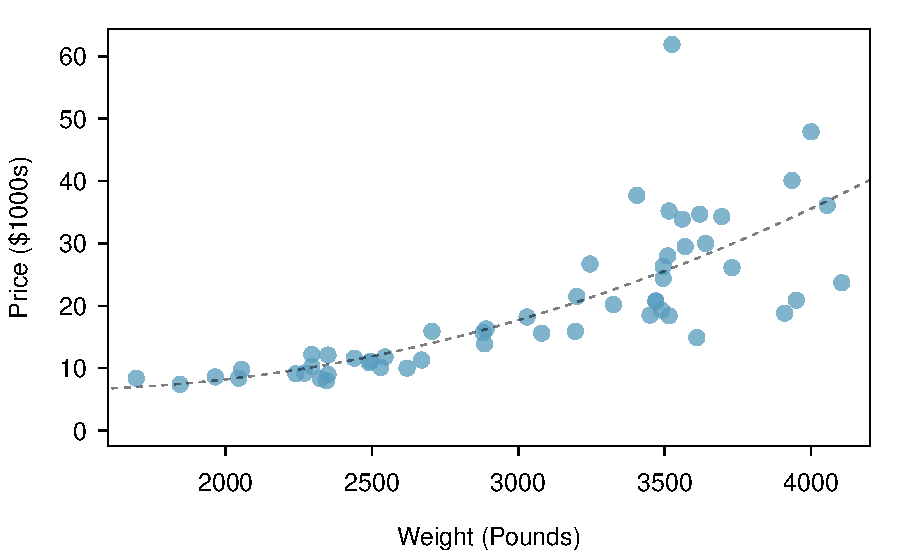
\includegraphics[width=0.8\textwidth]{ch_intro_to_data/figures/carsPriceVsWeight/carsPriceVsWeight}
   \caption{A scatterplot of \var{price} versus \var{weight} for 54 cars.}
   \label{carsPriceVsWeight}
\end{figure}
\end{example}
\index{data!cars|)}

\begin{exercise}
Describe two variables that would have a horseshoe shaped association in a scatterplot.\footnote{Consider the case where your vertical axis represents something ``good'' and your horizontal axis represents something that is only good in moderation. Health and water consumption fit this description since water becomes toxic when consumed in excessive quantities.}
\end{exercise}

\subsection{Dot plots and the mean}
\label{dotPlot}

Sometimes two variables are one too many: only one variable may be of interest. In these cases, a dot plot provides the most basic of displays. A~\term{dot plot} is a one-variable scatterplot; an example using the number of characters from 50 emails is shown in Figure~\ref{emailCharactersDotPlot}. A stacked version of this dot plot is shown in Figure~\ref{emailCharactersDotPlotStacked}.

\begin{figure}[h]
   \centering
   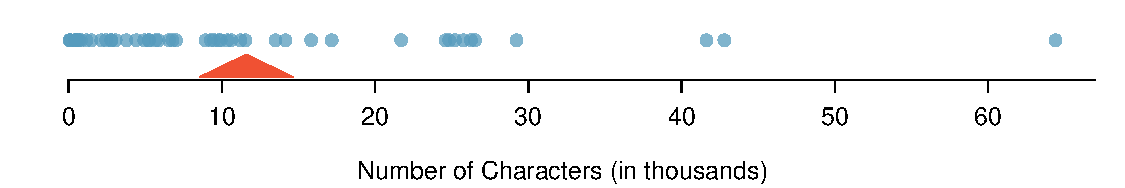
\includegraphics[width=\textwidth]{ch_intro_to_data/figures/emailCharactersDotPlot/emailCharactersDotPlot}
   \caption{A dot plot of \var{num\_\hspace{0.3mm}char} for the \data{email50} data set.}
   \label{emailCharactersDotPlot}
\end{figure}

\begin{figure}[h]
   \centering
   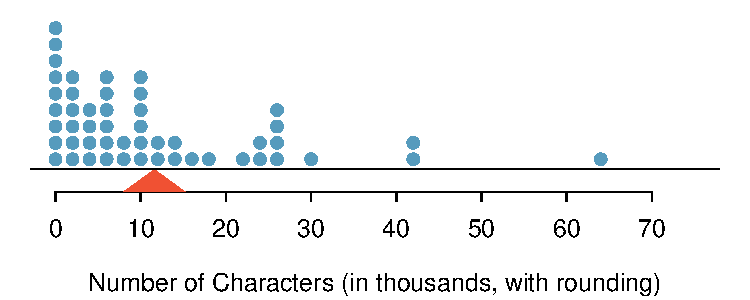
\includegraphics[width=0.72\textwidth]{ch_intro_to_data/figures/emailCharactersDotPlot/emailCharactersDotPlotStacked}
   \caption{A stacked dot plot of \var{num\_\hspace{0.3mm}char} for the \data{email50} data set. The~values have been rounded to the nearest 2,000 in this plot.}
   \label{emailCharactersDotPlotStacked}
\end{figure}

The \term{mean}, sometimes called the \indexthis{average}{mean!average}, is a common way to measure the center of a \term{distribution} of data. To find the mean number of characters in the 50 emails, we add up all the character counts and divide by the number of emails. For computational convenience, the number of characters is listed in the thousands and rounded to the first~decimal.
\begin{eqnarray}
\bar{x} = \frac{21.7 + 7.0 + \cdots + 15.8}{50} = 11.6
\label{sampleMeanEquation}
\end{eqnarray}
The sample mean is often labeled $\bar{x}$\marginpar[\raggedright$\bar{x}$\\\footnotesize sample\\ mean]{\raggedright$\bar{x}$\\\footnotesize sample\\ mean}. The letter $x$ is being used as a generic placeholder for the variable of interest, \var{num\_\hspace{0.3mm}char}, and the bar over on the $x$ communicates that the average number of characters in the 50 emails was 11,600. It is useful to think of the mean as the balancing point of the distribution. The sample mean is shown as a triangle in Figures~\ref{emailCharactersDotPlot} and~\ref{emailCharactersDotPlotStacked}.

\begin{termBox}{\tBoxTitle{Mean}%
The sample mean of a numerical variable is computed as the sum of all of the observations divided by the number of observations:
\begin{eqnarray}
\bar{x} = \frac{x_1+x_2+\cdots+x_n}{n}
\label{meanEquation}
\end{eqnarray}
where $x_1, x_2, \dots, x_n$ represent the $n$ observed values.}
\end{termBox}\marginpar[\raggedright\vspace{-8mm}

$n$\\\footnotesize sample size]{\raggedright\vspace{-8mm}

$n$\\\footnotesize sample size}\vspace{-2mm}

\begin{exercise}
Examine Equations~\eqref{sampleMeanEquation} and~\eqref{meanEquation} above. What does $x_1$ correspond to? And $x_2$? Can you infer a general meaning to what $x_i$ might represent?\footnote{$x_1$ corresponds to the number of characters in the first email in the sample (21.7, in thousands), $x_2$ to the number of characters in the second email (7.0, in thousands), and $x_i$ corresponds to the number of characters in the $i^{th}$ email in the data set.}
\end{exercise}

\begin{exercise}
What was $n$ in this sample of emails?\footnote{The sample size was $n=50$.}
\end{exercise}

The \data{email50} data set represents a sample from a larger population of emails that were received in January and March. We could compute a mean for this population in the same way as the sample mean, however, the population mean has a special label: $\mu$\marginpar[\raggedright$\mu$\\\footnotesize population\\ mean]{\raggedright$\mu$\\\footnotesize population\\ mean}. \index{Greek!mu@mu ($\mu$)} The symbol $\mu$ is the Greek letter \emph{mu} and represents the average of all observations in the population. Sometimes a subscript, such as $_x$, is used to represent which variable the population mean refers to, e.g. $\mu_x$.

\begin{example}{The average number of characters across all emails can be estimated using the sample data. Based on the sample of 50 emails, what would be a reasonable estimate of $\mu_x$, the mean number of characters in all emails in the \data{email} data set? (Recall that \data{email50} is a sample from \data{email}.)}
The sample mean, 11,600, may provide a reasonable estimate of $\mu_x$. While this number will not be perfect, it provides a \emph{point estimate} of the population mean. In Chapter~\ref{foundationsForInference} and beyond, we will develop tools to characterize the accuracy of point estimates, and we will find that point estimates based on larger samples tend to be more accurate than those based on smaller samples.
\end{example}

\begin{example}{We might like to compute the average income per person in the US. To do so, we might first think to take the mean of the per capita incomes across the 3,143 counties in the \data{county} data set. What would be a better approach?} \label{wtdMeanOfIncome}
The \data{county} data set is special in that each county actually represents many individual people. If we were to simply average across the \var{income} variable, we would be treating counties with 5,000 and 5,000,000 residents equally in the calculations. Instead, we should compute the total income for each county, add up all the counties' totals, and then divide by the number of people in all the counties. If we completed these steps with the \data{county} data, we would find that the per capita income for the US is \$27,348.43. Had we computed the \emph{simple} mean of per capita income across counties, the result would have been just \$22,504.70!
\end{example}

Example~\ref{wtdMeanOfIncome} used what is called a \term{weighted mean}\index{mean!weighted mean}, which will not be a key topic in this textbook. However, we have provided an online supplement on weighted means for interested readers:
\begin{center}
\oiRedirect{textbook-weighted_mean_supplement}{www.openintro.org/stat/down/supp/wtdmean.pdf}
\end{center}

\subsection{Histograms and shape}
\label{histogramsAndShape}

Dot plots show the exact value for each observation. This is useful for small data sets, but they can become hard to read with larger samples. Rather than showing the value of each observation, we prefer to think of the value as belonging to a \emph{bin}. For example, in the \data{email50} data set, we create a table of counts for the number of cases with character counts between 0 and 5,000, then the number of cases between 5,000 and 10,000, and so on. Observations that fall on the boundary of a bin (e.g. 5,000) are allocated to the lower bin. This tabulation is shown in Table~\ref{binnedNumCharTable}. These binned counts are plotted as bars in Figure~\ref{email50NumCharHist} into what is called a \term{histogram}, which resembles the stacked dot plot shown in Figure~\ref{emailCharactersDotPlotStacked}.

\begin{table}[ht]
\centering\small
\begin{tabular}{l ccc ccc ccc c}
  \hline
Characters & \\
(in thousands) & \raisebox{1.5ex}[0pt]{0-5} & \raisebox{1.5ex}[0pt]{5-10} & \raisebox{1.5ex}[0pt]{10-15} & \raisebox{1.5ex}[0pt]{15-20} & \raisebox{1.5ex}[0pt]{20-25} & \raisebox{1.5ex}[0pt]{25-30} & \raisebox{1.5ex}[0pt]{$\cdots$} & \raisebox{1.5ex}[0pt]{55-60} & \raisebox{1.5ex}[0pt]{60-65} \\
  \hline
Count & 19 & 12 & 6 & 2 & 3 & 5 & $\cdots$ & 0 & 1 \\
  \hline
\end{tabular}
\caption{The counts for the binned \var{num\_\hspace{0.3mm}char} data.}
\label{binnedNumCharTable}
\end{table}

\begin{figure}[bth]
   \centering
   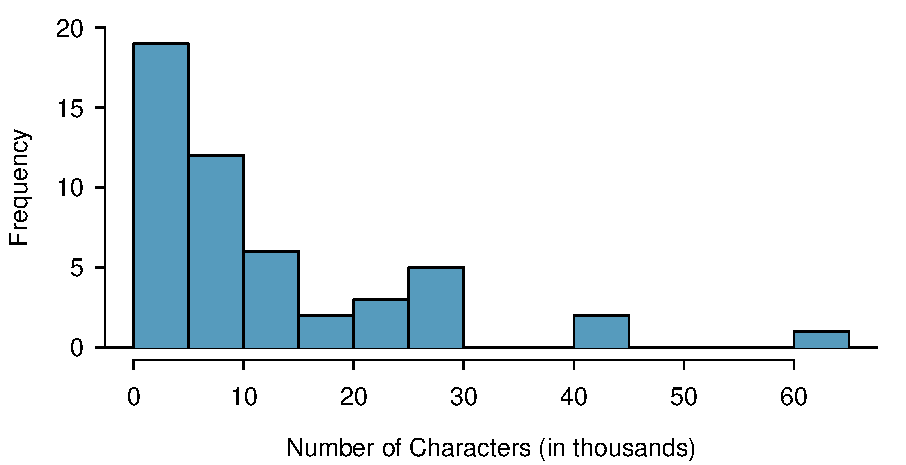
\includegraphics[width=0.82\textwidth]{ch_intro_to_data/figures/email50NumCharHist/email50NumCharHist}
   \caption{A histogram of \var{num\_\hspace{0.3mm}char}. This distribution is very strongly skewed to the right.\index{skew!example: very strong}}
   \label{email50NumCharHist}
\end{figure}

Histograms provide a view of the \term{data density}. Higher bars represent where the data are relatively more common. For instance, there are many more emails with fewer than 20,000 characters than emails with at least 20,000 in the data set. The bars make it easy to see how the density of the data changes relative to the number of characters.

Histograms are especially convenient for describing the shape of the data distribution\label{shapeFirstDiscussed}. Figure~\ref{email50NumCharHist} shows that most emails have a relatively small number of characters, while fewer emails have a very large number of characters. When data trail off to the right in this way and have a longer right \hiddenterm{tail}\index{skew!tail}, the shape is said to be \termsub{right skewed}{skew!right skewed}.\footnote{Other ways to describe data that are skewed to the right: \termni{skewed to the right}, \termni{skewed to the high end}, or \termni{skewed to the positive end}.}

Data sets with the reverse characteristic -- a long, thin tail to the left -- are said to be \termsub{left skewed}{skew!left skewed}. We also say that such a distribution has a long left tail. Data sets that show roughly equal trailing off in both directions are called \term{symmetric}.\index{skew!symmetric}

\begin{termBox}{\tBoxTitle{Long tails to identify skew}%
When data trail off in one direction, the distribution has a \term{long tail}. \index{skew!long tail|textbf} If a distribution has a long left tail, it is left skewed. If a distribution has a long right tail, it is right skewed.}
\end{termBox}

\begin{exercise}
Take a look at the dot plots in Figures~\ref{emailCharactersDotPlot} and~\ref{emailCharactersDotPlotStacked}. Can you see the skew in the data? Is it easier to see the skew in this histogram or the dot plots?\footnote{The skew is visible in all three plots, though the flat dot plot is the least useful. The stacked dot plot and histogram are helpful visualizations for identifying skew.}
\end{exercise}

\begin{exercise}
Besides the mean (since it was labeled), what can you see in the dot plots that you cannot see in the histogram?\footnote{Character counts for individual emails.}
\end{exercise}

In addition to looking at whether a distribution is skewed or symmetric, histograms can be used to identify modes. A \term{mode} is represented by a prominent peak in the distribution.\footnote{Another definition of mode, which is not typically used in statistics, is the value with the most occurrences. It is common to have \emph{no} observations with the same value in a data set, which makes this other definition useless for many real data sets.} There is only one prominent peak in the histogram of \var{num\_\hspace{0.3mm}char}.

Figure~\ref{singleBiMultiModalPlots} shows histograms that have one, two, or three prominent peaks. Such distributions are called \termsub{unimodal}{modality!unimodal}, \termsub{bimodal}{modality!bimodal}, and \termsub{multimodal}{modality!multimodal}, respectively. Any distribution with more than 2 prominent peaks is called multimodal. Notice that there was one prominent peak in the unimodal distribution with a second less prominent peak that was not counted since it only differs from its neighboring bins by a few observations.

\begin{figure}[h]
   \centering
   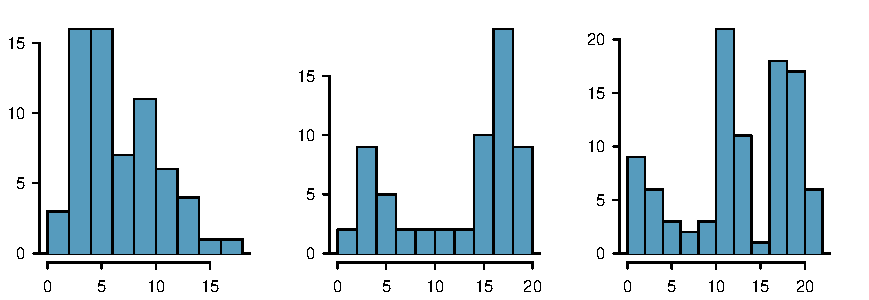
\includegraphics[width=\textwidth]{ch_intro_to_data/figures/singleBiMultiModalPlots/singleBiMultiModalPlots}
   \caption{Counting only prominent peaks, the distributions are (left to right) unimodal, bimodal, and multimodal.}
   \label{singleBiMultiModalPlots}
\end{figure}

\begin{exercise}
Figure~\ref{email50NumCharHist} reveals only one prominent mode in the number of characters. Is the distribution unimodal, bimodal, or multimodal?\footnote{Unimodal. Remember that \emph{uni} stands for 1 (think \emph{uni}cycles). Similarly, \emph{bi} stands for~2 (think \emph{bi}cycles). (We're hoping a \emph{multicycle} will be invented to complete this analogy.)}
\end{exercise}

\begin{exercise}
Height measurements of young students and adult teachers at a K-3 elementary school were taken. How many modes would you anticipate in this height data set?\footnote{There might be two height groups visible in the data set: one of the students and one of the adults. That is, the data are probably bimodal.}
\end{exercise}

\begin{tipBox}{\tipBoxTitle{Looking for modes}
Looking for modes isn't about finding a clear and correct answer about the number of modes in a distribution, which is why \emph{prominent} is not rigorously defined in this book. The important part of this examination is to better understand your data and how it might be structured.}
\end{tipBox}


\subsection{Variance and standard deviation}
\label{variability}

The mean was introduced as a method to describe the center of a data set, but the \indexthis{variability}{variability} in the data is also important. Here, we introduce two measures of variability: the variance and the standard deviation. Both of these are very useful in data analysis, even though their formulas are a bit tedious to calculate by hand. The standard deviation is the easier of the two to understand, and it roughly describes how far away the typical observation is from the mean.

We call the distance of an observation from its mean its \term{deviation}. Below are the deviations for the $1^{st}_{}$, $2^{nd}_{}$, $3^{rd}$, and $50^{th}_{}$ observations in the \var{num\_\hspace{0.3mm}char} variable. For computational convenience, the number of characters is listed in the thousands and rounded to the first decimal.
\begin{align*}
x_1^{}-\bar{x} &= 21.7 - 11.6 = 10.1 \hspace{5mm}\text{ } \\
x_2^{}-\bar{x} &= 7.0 - 11.6 = -4.6 \\
x_3^{}-\bar{x} &= 0.6 - 11.6 = -11.0 \\
			&\ \vdots \\
x_{50}^{}-\bar{x} &= 15.8 - 11.6 = 4.2
\end{align*}
% library(openintro); d <- email50$num_char; round(mean(d),1); d[c(1,2,3,50)]; d[c(1,2,3,50)] - round(mean(d),1); (d[c(1,2,3,50)] - round(mean(d)))^2; sum((d - round(mean(d)))^2)/49; sqrt(sum((d - round(mean(d)))^2)/49); var(d); sd(d)
If we square these deviations and then take an average, the result is about equal to the sample \term{variance}\label{varianceIsDefined}, denoted by $s_{}^2$\marginpar[\raggedright$s^2_{}$\\\footnotesize sample variance]{\raggedright$s^2_{}$\\\footnotesize sample variance}:
\begin{align*}
s_{}^2 &= \frac{10.1_{}^2 + (-4.6)_{}^2 + (-11.0)_{}^2 + \cdots + 4.2_{}^2}{50-1} \\
	&= \frac{102.01 + 21.16 + 121.00 + \cdots + 17.64}{49} \\
	&= 172.44
\end{align*}
We divide by $n-1$, rather than dividing by $n$, when computing the variance; you need not worry about this mathematical nuance for the material in this textbook. Notice that squaring the deviations does two things. First, it makes large values much larger, seen by comparing $10.1^2$, $(-4.6)^2$, $(-11.0)^2$, and $4.2^2$. Second, it gets rid of any negative signs.

The \term{standard deviation} is defined as the square root of the variance:
$$s=\sqrt{172.44} = 13.13$$
\marginpar[\raggedright\vspace{-10mm}

$s$\\\footnotesize sample standard deviation]{\raggedright\vspace{-10mm}

$s$\\\footnotesize sample standard deviation
}\index{s@$s$}The standard deviation of the number of characters in an email is about 13.13 thousand. A subscript of $_x$ may be added to the variance and standard deviation, i.e. $s_x^2$ and $s_x^{}$, as a reminder that these are the variance and standard deviation of the observations represented by $x_1^{}$, $x_2^{}$, ..., $x_n^{}$. The $_{x}$ subscript is usually omitted when it is clear which data the variance or standard deviation is referencing.

\begin{termBox}{\tBoxTitle{Variance and standard deviation}
The variance is roughly the average squared distance from the mean. The standard deviation is the square root of the variance. The standard deviation is useful when considering how close the data are to the mean.}
\end{termBox}

Formulas and methods used to compute the variance and standard deviation for a population are similar to those used for a sample.\footnote{The only difference is that the population variance has a division by $n$ instead of $n-1$.} However, like the mean, the population values have special symbols: $\sigma_{}^2$\marginpar[\raggedright$\sigma_{}^2$\\\footnotesize population variance\\ \hspace{2mm}]{\raggedright$\sigma_{}^2$\\\footnotesize population variance\\ \hspace{2mm}} for the variance and $\sigma$\marginpar[\raggedright$\sigma$\\\footnotesize population standard deviation\\ \hspace{2mm}]{\raggedright$\sigma$\\\footnotesize population standard deviation\\ \hspace{2mm}} for the standard deviation. The symbol $\sigma$ \index{Greek!sigma@sigma ($\sigma$)} is the Greek letter \emph{sigma}.


\begin{figure}
\centering
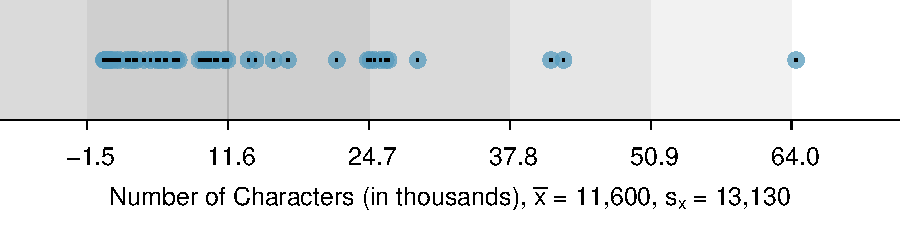
\includegraphics[width=\mycaptionwidth]{ch_intro_to_data/figures/sdAsRuleForEmailNumChar/sdAsRuleForEmailNumChar}
\caption{In the \var{num\_\hspace{0.3mm}char} data, 41 of the 50 emails (82\%) are within 1~standard deviation of the mean, and 47 of the 50 emails (94\%) are within 2 standard deviations. Usually about 70\% of the data are within 1 standard deviation of the mean and 95\% are within 2 standard deviations, though this rule of thumb is less accurate for skewed data, as shown in this example.}
\label{sdAsRuleForEmailNumChar}
\end{figure}

\begin{tipBox}{\tipBoxTitle{standard deviation describes variability}
Focus on the conceptual meaning of the standard deviation as a descriptor of variability rather than the formulas. Usually 70\% of the data will be within one standard deviation of the mean and about 95\% will be within two standard deviations. However, as seen in Figures~\ref{sdAsRuleForEmailNumChar} and~\ref{severalDiffDistWithSdOf1}, these percentages are not strict rules.}
\end{tipBox}

\begin{figure}
\centering
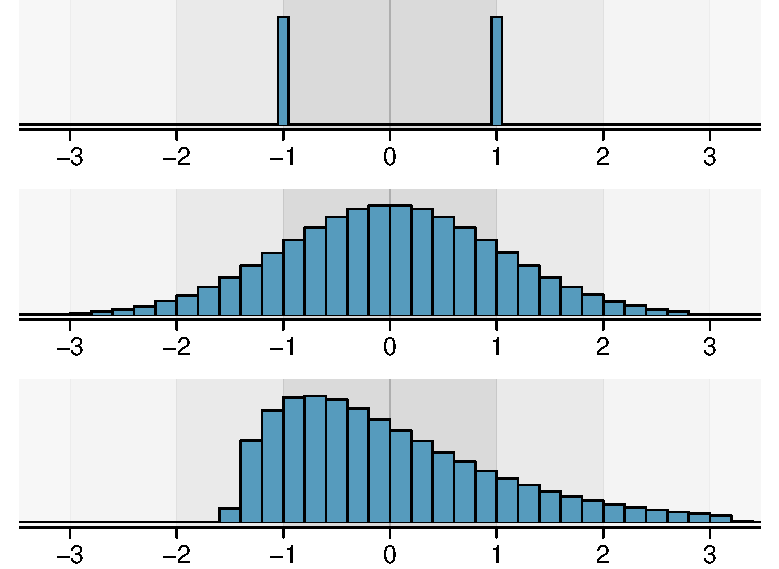
\includegraphics[width=0.64\textwidth]{ch_intro_to_data/figures/severalDiffDistWithSdOf1/severalDiffDistWithSdOf1}
\caption{Three very different population distributions with the same mean $\mu=0$ and standard deviation $\sigma=1$.}
\label{severalDiffDistWithSdOf1}
\end{figure}

\begin{exercise}
On page~\pageref{shapeFirstDiscussed}, the concept of shape of a distribution was introduced. A good description of the shape of a distribution should include modality and whether the distribution is symmetric or skewed to one side. Using Figure~\ref{severalDiffDistWithSdOf1} as an example, explain why such a description is important.\footnote{Figure~\ref{severalDiffDistWithSdOf1} shows three distributions that look quite different, but all have the same mean, variance, and standard deviation. Using modality, we can distinguish between the first plot (bimodal) and the last two (unimodal). Using skewness, we can distinguish between the last plot (right skewed) and the first two. While a picture, like a histogram, tells a more complete story, we can use modality and shape (symmetry/skew) to characterize basic information about a~distribution.}
\end{exercise}

\begin{example}{Describe the distribution of the \var{num\_\hspace{0.3mm}char} variable using the histogram in Figure~\vref{email50NumCharHist}. The description should incorporate the center, variability, and shape of the distribution, and it should also be placed in context: the number of characters in emails. Also note any especially unusual cases.}
The distribution of email character counts is unimodal and very strongly skewed to the high end. Many of the counts fall near the mean at 11,600, and most fall within one standard deviation (13,130) of the mean. There is one exceptionally long email with about 65,000 characters.
\end{example}

In practice, the variance and standard deviation are sometimes used as a means to an end, where the ``end'' is being able to accurately estimate the uncertainty associated with a sample statistic. For example, in Chapter~\ref{foundationsForInference} we will use the variance and standard deviation to assess how close the sample mean is to the population mean.

\subsection{Box plots, quartiles, and the median}

A \term{box plot} summarizes a data set using five statistics while also plotting unusual observations. Figure~\ref{boxPlotLayoutNumVar} provides a vertical dot plot alongside a box plot of the \var{num\_\hspace{0.3mm}char} variable from the \data{email50} data set.

\begin{figure}[h]
   \centering
   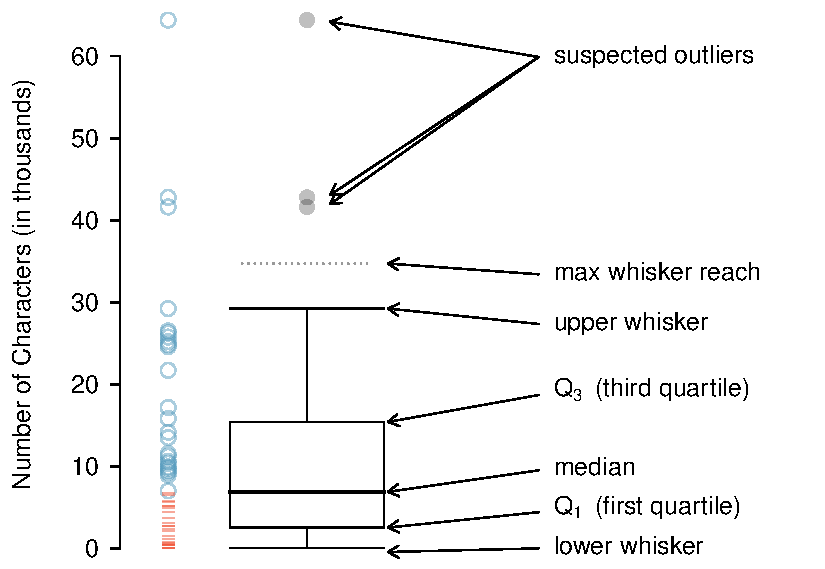
\includegraphics[width=0.86\mycaptionwidth]{ch_intro_to_data/figures/boxPlotLayoutNumVar/boxPlotLayoutNumVar}
   \caption{A vertical dot plot next to a labeled box plot for the number of characters in 50 emails. The median (6,890), splits the data into the bottom 50\% and the top 50\%, marked in the dot plot by horizontal dashes and open circles, respectively.}
   \label{boxPlotLayoutNumVar}
\end{figure}

The first step in building a box plot is drawing a dark line denoting the \term{median}, which splits the data in half. Figure~\ref{boxPlotLayoutNumVar} shows 50\% of the data falling below the median (dashes) and other 50\% falling above the median (open circles). There are 50 character counts in the data set (an even number) so the data are perfectly split into two groups of~25. We take the median in this case to be the average of the two observations closest to the $50^{th}$ percentile: $(\text{6,768} + \text{7,012}) / 2 = \text{6,890}$. When there are an odd number of observations, there will be exactly one observation that splits the data into two halves, and in this case that observation is the median (no average needed).

\begin{termBox}{\tBoxTitle{Median: the number in the middle}
If the data are ordered from smallest to largest, the \term{median} is the observation right in the middle. If there are an even number of observations, there will be two values in the middle, and the median is taken as their average.}
\end{termBox}

The second step in building a box plot is drawing a rectangle to represent the middle 50\% of the data. The total length of the box, shown vertically in Figure~\ref{boxPlotLayoutNumVar}, is called the \term{interquartile range} (\hiddenterm{IQR}, for short). It, like the standard deviation, is a measure of \indexthis{variability}{variability} in data. The more variable the data, the larger the standard deviation and~IQR. The two boundaries of the box are called the \term{first quartile} \index{quartile!first quartile} (the $25^{th}$ \hiddenterm{percentile}, i.e. 25\% of the data fall below this value) and the \term{third quartile} \index{quartile!third quartile} (the $75^{th}$ percentile), and these are often labeled $Q_1$ \index{Q$_1$} and $Q_3$\index{Q$_3$}, respectively.

\begin{termBox}{\tBoxTitle{Interquartile range (IQR)}
The IQR\index{interquartile range} is the length of the box in a box plot. It is computed as
\begin{eqnarray*}
IQR = Q_3 - Q_1
\end{eqnarray*}
where $Q_1$ and $Q_3$ are the $25^{th}$ and $75^{th}$ percentiles.}
\end{termBox}

\begin{exercise}
What percent of the data fall between $Q_1$ and the median? What percent is between the median and $Q_3$?\footnote{Since $Q_1$ and $Q_3$ capture the middle 50\% of the data and the median splits the data in the middle, 25\% of the data fall between $Q_1$ and the median, and another 25\% falls between the median and $Q_3$.}
\end{exercise}

Extending out from the box, the \term{whiskers} attempt to capture the data outside of the box, however, their reach is never allowed to be more than $1.5\times IQR$.\footnote{While the choice of exactly 1.5 is arbitrary, it is the most commonly used value for box plots.} They capture everything within this reach. In Figure~\ref{boxPlotLayoutNumVar}, the upper whisker does not extend to the last three points, which is beyond $Q_3 + 1.5\times IQR$, and so it extends only to the last point below this limit. The lower whisker stops at the lowest value, 33, since there is no additional data to reach; the lower whisker's limit is not shown in the figure because the plot does not extend down to $Q_1 - 1.5\times IQR$. In a sense, the box is like the body of the box plot and the whiskers are like its arms trying to reach the rest of the data.

Any observation that lies beyond the whiskers is labeled with a dot. The purpose of labeling these points -- instead of just extending the whiskers to the minimum and maximum observed values -- is to help identify any observations that appear to be unusually distant from the rest of the data. Unusually distant observations are called \termsub{outliers}{outlier}. In this case, it would be reasonable to classify the emails with character counts of 41,623, 42,793, and 64,401 as outliers since they are numerically distant from most of the data.

\begin{termBox}{\tBoxTitle{Outliers are extreme}
An \term{outlier} is an observation that appears extreme relative to the rest of the data.}
\end{termBox}


\begin{tipBox}{\tipBoxTitle{Why it is important to look for outliers}
Examination of data for possible outliers serves many useful purposes, including\vspace{-2mm}
\begin{enumerate}
\setlength{\itemsep}{0mm}
\item Identifying \indexthis{strong skew}{skew!example: strong} in the distribution.
\item Identifying data collection or entry errors. For instance, we re-examined the email purported to have 64,401 characters to ensure this value was accurate.
\item Providing insight into interesting properties of the data.\vspace{0.5mm}
\end{enumerate}}
\end{tipBox}

\begin{exercise}
The observation 64,401, a suspected outlier, was found to be an accurate observation. What would such an observation suggest about the nature of character counts in emails?\footnote{That occasionally there may be very long emails.}\end{exercise}

\begin{exercise}
Using Figure~\ref{boxPlotLayoutNumVar}, estimate the following values for \var{num\_\hspace{0.3mm}char} in the \data{email50} data set: (a) $Q_1$, (b) $Q_3$, and (c) IQR.\footnote{These visual estimates will vary a little from one person to the next: $Q_1=$ 3,000, $Q_3=$ 15,000, $\text{IQR}=Q_3 - Q_1 = $ 12,000. (The true values: $Q_1=$ 2,536, $Q_3=$ 15,411, $\text{IQR} = $ 12,875.)}
\end{exercise}

\CalculatorVideos{how to create statistical summaries and box plots}


\subsection{Robust statistics}

How are the \indexthis{sample statistics}{sample statistic} of the \data{num\_\hspace{0.3mm}char} data set affected by the observation, 64,401? What would have happened if this email wasn't observed? What would happen to these \indexthis{summary statistics}{summary statistic} if the observation at 64,401 had been even larger, say 150,000? These scenarios are plotted alongside the original data in Figure~\ref{email50NumCharDotPlotRobustEx}, and sample statistics are computed under each scenario in Table~\ref{robustOrNotTable}.

\begin{figure}[ht]
\centering
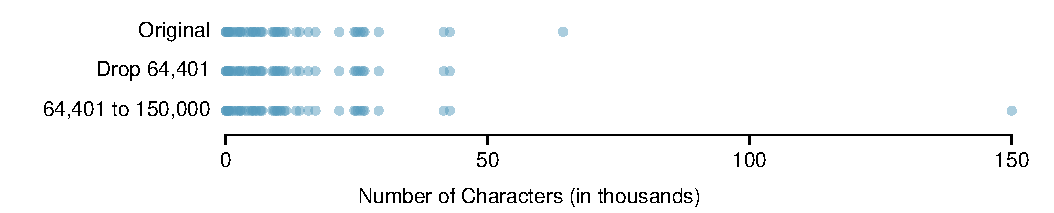
\includegraphics[width=\textwidth]{ch_intro_to_data/figures/email50NumCharDotPlotRobustEx/email50NumCharDotPlotRobustEx}
\caption{Dot plots of the original character count data and two modified data sets.}
\label{email50NumCharDotPlotRobustEx}
\end{figure}

\begin{table}[ht]
\centering
\begin{tabular}{l c cc c cc}
  \hline
& \hspace{0mm} & \multicolumn{2}{c}{\bf robust} & \hspace{2mm} & \multicolumn{2}{c}{\bf not robust} \\
scenario && median & IQR && $\bar{x}$ & $s$ \\ 
  \hline
original \var{num\_\hspace{0.3mm}char} data 	&& 6,890 & 12,875 && 11,600 & 13,130 \\
% library(openintro); data(email50); d <- email50$num_char; median(d); diff(quantile(d, c(0.25,0.75))); mean(d); sd(d)
drop 66,924 observation		&& 6,768 & 11,702 && 10,521 & 10,798 \\
% library(openintro); data(email50); d <- email50$num_char; d <- d[-which.max(d)]; median(d); diff(quantile(d, c(0.25,0.75))); mean(d); sd(d)
move 66,924 to 150,000		&& 6,890 & 12,875 && 13,310 & 22,434 \\
% library(openintro); data(email50); d <- email50$num_char; d[which.max(d)] <- 100000; median(d); diff(quantile(d, c(0.25,0.75))); mean(d); sd(d)
   \hline
\end{tabular}
\caption{A comparison of how the median, IQR, mean ($\bar{x}$), and standard deviation ($s$) change when extreme observations are present.}
\label{robustOrNotTable}
\end{table}

\begin{exercise} \label{numCharWhichIsMoreRobust}
(a) Which is more affected by extreme observations, the mean or median? Table~\ref{robustOrNotTable} may be helpful. (b) Is the standard deviation or IQR more affected by extreme observations?\footnote{(a) Mean is affected more. (b) Standard deviation is affected more. Complete explanations are provided in the material following Guided Practice~\ref{numCharWhichIsMoreRobust}.}
\end{exercise}

The median and IQR are called \term{robust estimates} because extreme observations have little effect on their values. The mean and standard deviation are much more affected by changes in extreme observations.

\begin{example}{The median and IQR do not change much under the three scenarios in Table~\ref{robustOrNotTable}. Why might this be the case?}
The median and IQR are only sensitive to numbers near $Q_1$, the median, and $Q_3$. Since values in these regions are relatively stable -- there aren't large jumps between observations -- the median and IQR estimates are also quite stable.
\end{example}

\begin{exercise}
The distribution of vehicle prices tends to be right skewed, with a few luxury and sports cars lingering out into the right tail. If you were searching for a new car and cared about price, should you be more interested in the mean or median price of vehicles sold, assuming you are in the market for a regular car?\footnote{Buyers of a ``regular car'' should be concerned about the median price. High-end car sales can drastically inflate the mean price while the median will be more robust to the influence of those sales.}
\end{exercise}

\subsection{Transforming data (special topic)}
\label{transformingDataSubsection}

When data are very strongly skewed, we sometimes transform them so they are easier to model. Consider the histogram of salaries for Major League Baseball players' salaries from 2010, which is shown in Figure~\ref{histMLBSalariesReg}.

\begin{figure}[ht]
\centering
\subfigure[]{
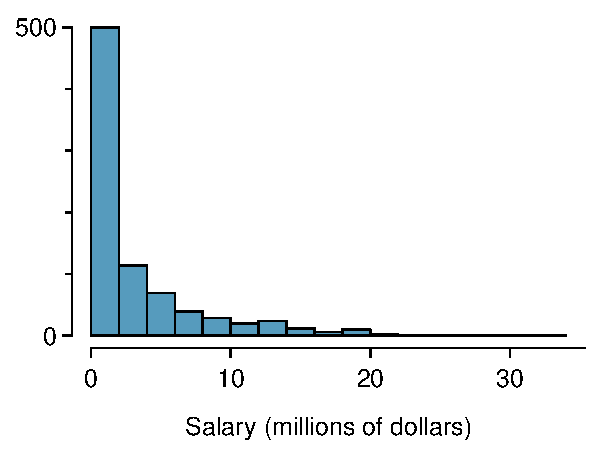
\includegraphics[width=0.46\textwidth]{ch_intro_to_data/figures/histMLBSalaries/histMLBSalariesReg}
\label{histMLBSalariesReg}
}
\subfigure[]{
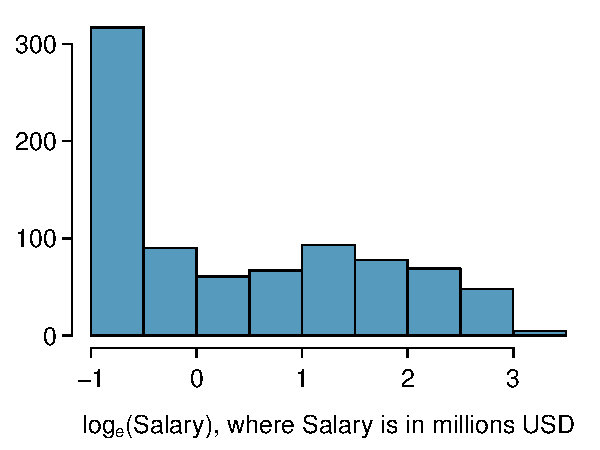
\includegraphics[width=0.46\textwidth]{ch_intro_to_data/figures/histMLBSalaries/histMLBSalariesLog}
\label{histMLBSalariesLog}
}
\caption{\subref{histMLBSalariesReg} Histogram of MLB player salaries for 2010, in millions of dollars. \subref{histMLBSalariesLog} Histogram of the log-transformed MLB player salaries for 2010.}
\label{histMLBSalaries}
\end{figure}

\begin{example}{The histogram of MLB player salaries is useful in that we can see the data are extremely skewed\index{skew!example: extreme} and centered (as gauged by the median) at about \$1 million. What isn't useful about this plot?}
Most of the data are collected into one bin in the histogram and the data are so strongly skewed that many details in the data are obscured.
\end{example}

There are some standard transformations that are often applied when much of the data cluster near zero (relative to the larger values in the data set) and all observations are positive. A \term{transformation} is a rescaling of the data using a function. For instance, a plot of the natural logarithm\footnote{Statisticians often write the natural logarithm as $\log$. You might be more familiar with it being written as $\ln$.} of player salaries results in a new histogram in Figure~\ref{histMLBSalariesLog}. Transformed data are sometimes easier to work with when applying statistical models because the transformed data are much less skewed and outliers are usually less extreme.

Transformations can also be applied to one or both variables in a scatterplot. A scatterplot of the \var{line\_\hspace{0.3mm}breaks} and \var{num\_\hspace{0.3mm}char} variables is shown in Figure~\ref{email50LinesCharactersMod}, which was earlier shown in Figure~\ref{email50LinesCharacters}. We can see a positive association between the variables and that many observations are clustered near zero. In Chapter~\ref{linRegrForTwoVar}, we might want to use a straight line to model the data. However, we'll find that the data in their current state cannot be modeled very well. Figure~\ref{email50LinesCharactersModLog} shows a scatterplot where both the \var{line\_\hspace{0.3mm}breaks} and \var{num\_\hspace{0.3mm}char} variables have been transformed using a log (base $e$) transformation. While there is a positive association in each plot, the transformed data show a steadier trend, which is easier to model than the untransformed data.

\begin{figure}
\centering
\subfigure[]{
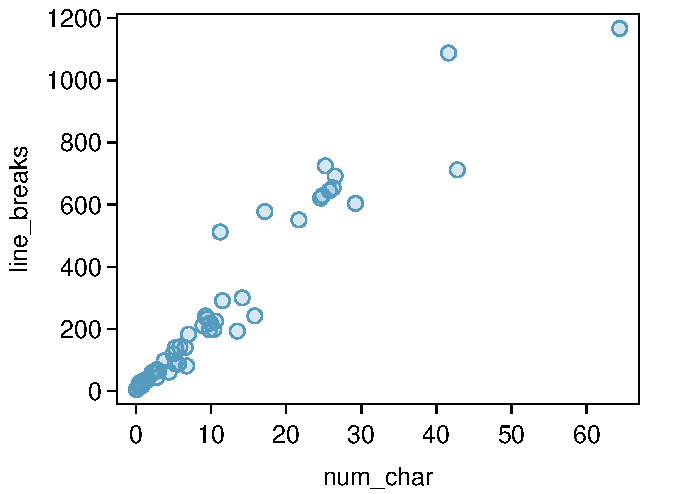
\includegraphics[width=0.47\textwidth]{ch_intro_to_data/figures/email50LinesCharactersMod/email50LinesCharactersMod}
\label{email50LinesCharactersMod}
}
\subfigure[]{
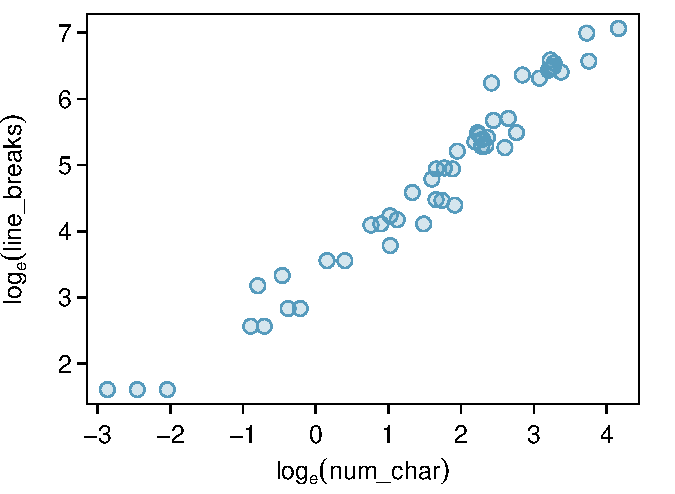
\includegraphics[width=0.47\textwidth]{ch_intro_to_data/figures/email50LinesCharactersMod/email50LinesCharactersModLog}
\label{email50LinesCharactersModLog}
}
\caption{\subref{email50LinesCharactersMod} Scatterplot of \var{line\_\hspace{0.3mm}breaks} against \var{num\_\hspace{0.3mm}char} for 50 emails. \subref{email50LinesCharactersModLog} A scatterplot of the same data but where each variable has been log-transformed.}
\label{email50LinesCharactersModMain}
\end{figure}

Transformations other than the logarithm can be useful, too. For instance, the square root ($\sqrt{\text{original observation}}$) and inverse ($\frac{1}{\text{original observation}}$) are used by statisticians. Common goals in transforming data are to see the data structure differently, reduce skew, assist in modeling, or straighten a nonlinear relationship in a scatterplot.

\index{data!email50|)}

\subsection{Mapping data (special topic)}

\index{data!county|(}
\index{intensity map|(}

The \data{county} data set offers many numerical variables that we could plot using dot plots, scatterplots, or box plots, but these miss the true nature of the data. Rather, when we encounter geographic data, we should map it using an \term{intensity map}, where colors are used to show higher and lower values of a variable. Figures~\ref{countyIntensityMaps1} and~\ref{countyIntensityMaps2} shows intensity maps for federal spending per capita (\var{fed\_\hspace{0.3mm}spend}), poverty rate in percent (\var{poverty}), homeownership rate in percent (\var{homeownership}), and median household income (\var{med\_\hspace{0.3mm}income}). The color key indicates which colors correspond to which values. Note that the intensity maps are not generally very helpful for getting precise values in any given county, but they are very helpful for seeing geographic trends and generating interesting research questions.

\begin{figure}
\centering
\subfigure[]{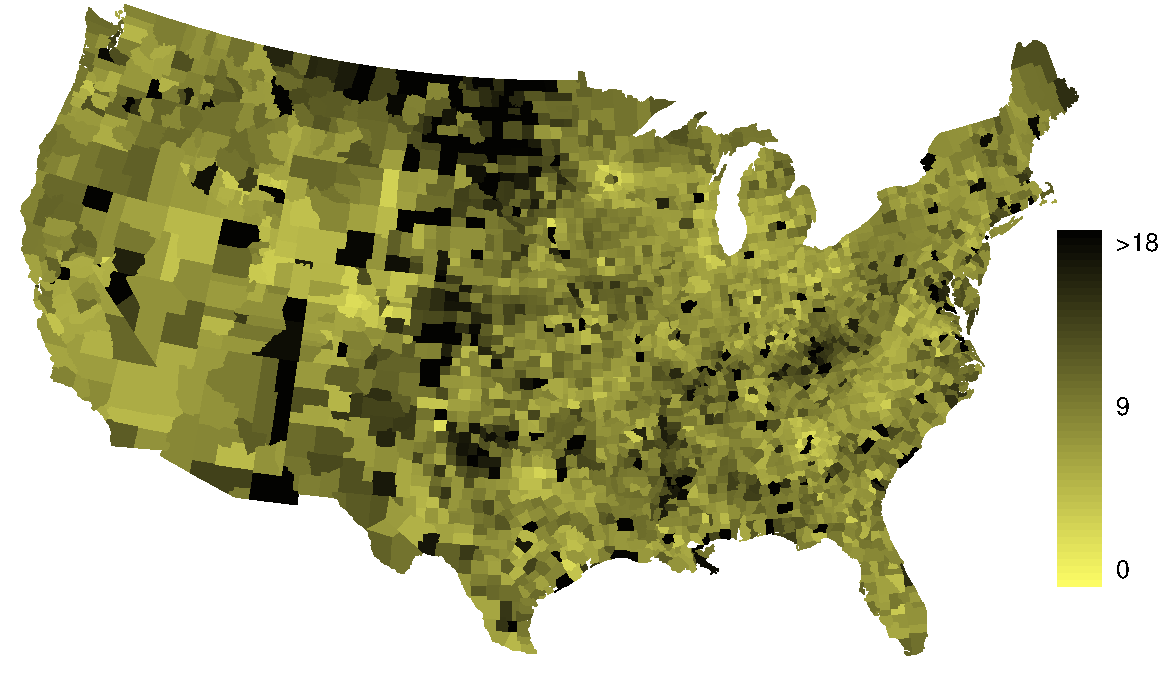
\includegraphics[width=\textwidth]{ch_intro_to_data/figures/countyIntensityMaps/countyFedSpendMap}\label{countyFedSpendMap}}
\subfigure[]{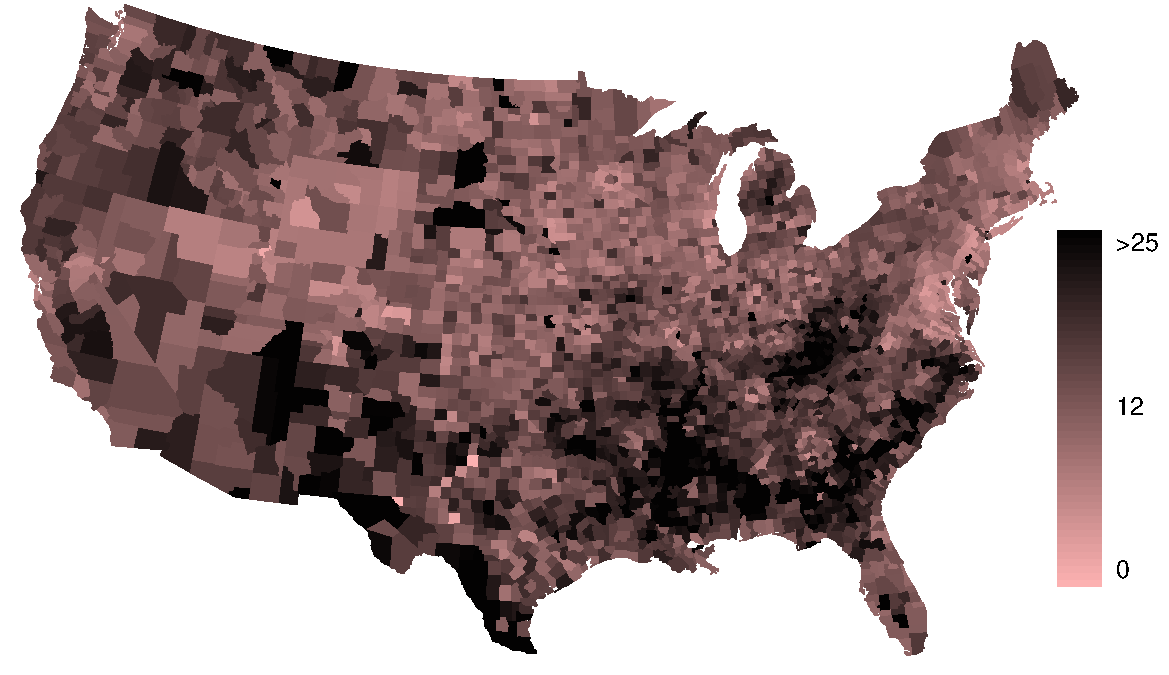
\includegraphics[width=\textwidth]{ch_intro_to_data/figures/countyIntensityMaps/countyPovertyMap}\label{countyPovertyMap}}
\caption{\subref{countyFedSpendMap} Map of federal spending (dollars per capita). \subref{countyPovertyMap} Intensity map of poverty rate (percent).}
\label{countyIntensityMaps1}
\end{figure}

\begin{figure}
\centering
\subfigure[]{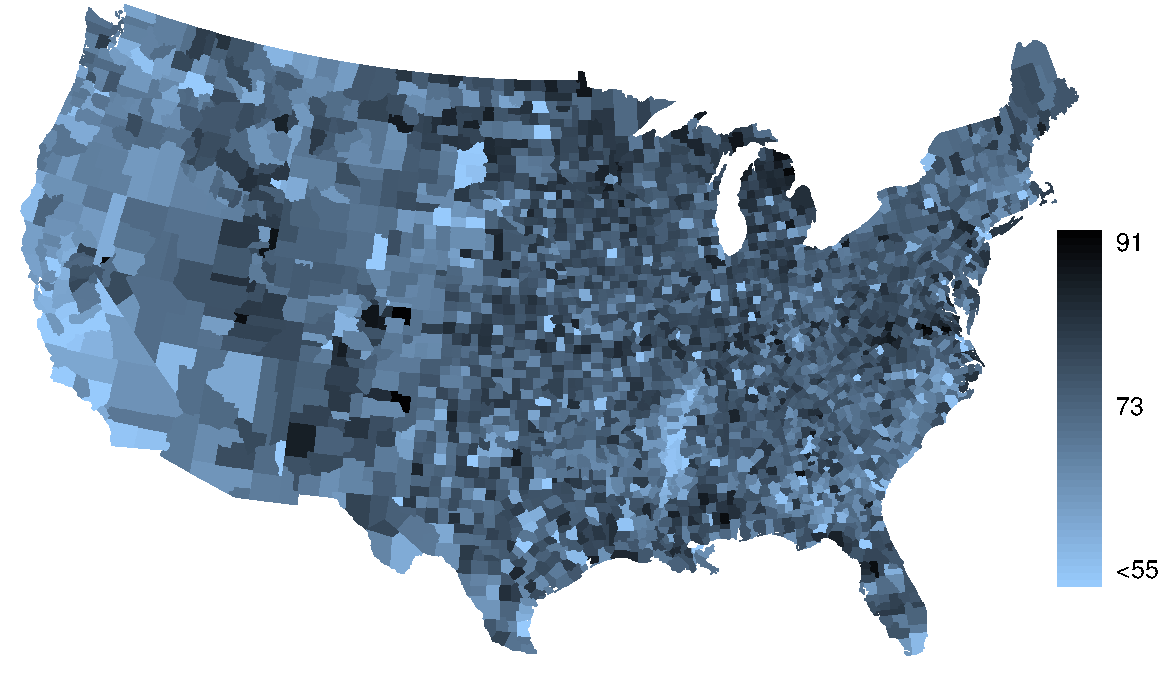
\includegraphics[width=\textwidth]{ch_intro_to_data/figures/countyIntensityMaps/countyHomeownershipMap}\label{countyHomeownershipMap}}
\subfigure[]{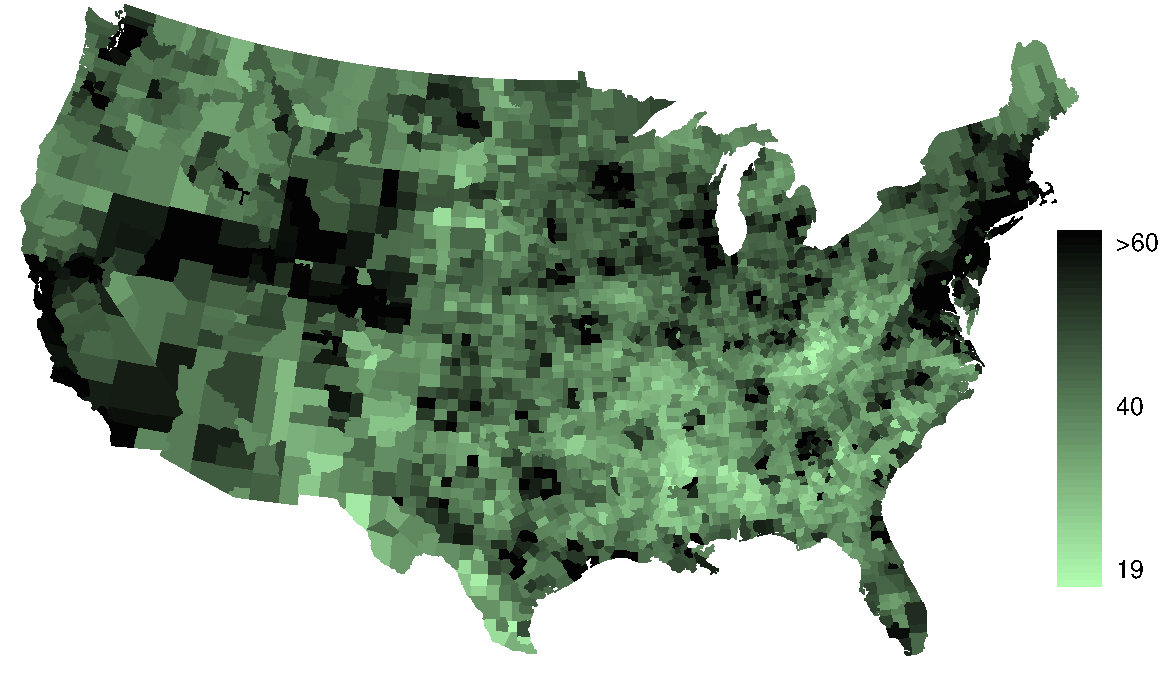
\includegraphics[width=\textwidth]{ch_intro_to_data/figures/countyIntensityMaps/countyMedIncomeMap}\label{countyMedIncomeMap}}
\caption{\subref{countyHomeownershipMap} Intensity map of homeownership rate (percent). \subref{countyMedIncomeMap} Intensity map of median household income (\$1000s).}
\label{countyIntensityMaps2}
\end{figure}

\textC{\pagebreak}

\begin{example}{What interesting features are evident in the \var{fed\_\hspace{0.3mm}spend} and \var{poverty} intensity maps?}
The federal spending intensity map shows substantial spending in the Dakotas and along the central-to-western part of the Canadian border, which may be related to the oil boom in this region. There are several other patches of federal spending, such as a vertical strip in eastern Utah and Arizona and the area where Colorado, Nebraska, and Kansas meet. There are also seemingly random counties with very high federal spending relative to their neighbors. If we did not cap the federal spending range at \$18 per capita, we would actually find that some counties have extremely high federal spending while there is almost no federal spending in the neighboring counties. These high-spending counties might contain military bases, companies with large government contracts, or other government facilities with many employees.

Poverty rates are evidently higher in a few locations. Notably, the deep south shows higher poverty rates, as does the southwest border of Texas. The vertical strip of eastern Utah and Arizona, noted above for its higher federal spending, also appears to have higher rates of poverty (though generally little correspondence is seen between the two variables).  High poverty rates are evident in the Mississippi flood plains a little north of New Orleans and also in a large section of Kentucky and West Virginia.
\end{example}

\begin{exercise}
What interesting features are evident in the \var{med\_\hspace{0.3mm}income} intensity map in Figure~\ref{countyMedIncomeMap}?\footnote{Note: answers will vary. There is a very strong correspondence between high earning and metropolitan areas. You might look for large cities you are familiar with and try to spot them on the map as dark spots.}
\end{exercise}

\index{intensity map|)}
\index{data!county|)}



\textC{\newpage}

\section[Considering categorical data]{Considering categorical data \sectionvideohref{youtube-7NhNeADL8fA&list=PLkIselvEzpM6pZ76FD3NoCvvgkj_p-dE8}}
\label{categoricalData}

\index{data!email|(}

Like numerical data, categorical data can also be organized and analyzed. In this section, we will introduce tables and other basic tools for categorical data that are used throughout this book. The \data{email50} data set represents a sample from a larger email data set called \data{email}. This larger data set contains information on 3,921 emails. In this section we will examine whether the presence of numbers, small or large, in an email provides any useful value in classifying email as spam or not spam.
% library(openintro); data(email); dim(email)

\subsection{Contingency tables and bar plots}

Table~\ref{emailSpamNumberTableTotals} summarizes two variables: \var{spam} and \var{number}. Recall that \var{number} is a categorical variable that describes whether an email contains no numbers, only small numbers (values under 1 million), or at least one big number (a value of 1 million or more). A table that summarizes data for two categorical variables in this way is called a \term{contingency table}. Each value in the table represents the number of times a particular combination of variable outcomes occurred. For example, the value 149 corresponds to the number of emails in the data set that are spam \emph{and} had no number listed in the email. Row and column totals are also included. The \term{row totals} \index{contingency table!row totals} provide the total counts across each row (e.g. $149 + 168 + 50 = 367$), and \term{column totals} \index{contingency table!column totals} are total counts down each column.

A table for a single variable is called a \term{frequency table}. Table~\ref{emailNumberTable} is a frequency table for the \var{number} variable. If we replaced the counts with percentages or proportions, the table would be called a \term{relative frequency table}.

\begin{table}[ht]
\centering
\begin{tabular}{ll  ccc  rr}
& & \multicolumn{3}{c}{\bf \var{number}} & \\
  \cline{3-5}
& & none & small & big & Total & \hspace{2mm}\  \\ 
  \cline{2-6}
	 & spam &  149 & 168 &  50 & 367 \\ 
\raisebox{1.5ex}[0pt]{\var{spam}} 
	& not spam &  400 & 2659 & 495 & 3554 \\ 
  \cline{2-6}
& Total & 549 & 2827 & 545 & 3921 \\
  \cline{2-6}
\end{tabular}
\caption{A contingency table for \var{spam} and \var{number}.}
\label{emailSpamNumberTableTotals}
%library(openintro); library(xtable); data(email); tab <- table(email[,c("spam", "number")])[2:1,]; xtable(tab); rowSums(tab); colSums(tab); sum(tab)
\end{table}

\begin{table}[htb]
\centering
\begin{tabular}{cccc}
  \hline
none & small & big & Total \\ 
 % \hline
 549 & 2827 & 545 & 3921 \\
   \hline
\end{tabular}
\caption{A frequency table for the \var{number} variable.}
\label{emailNumberTable}
\end{table}
%library(openintro); library(xtable); data(email); xtable(table(email[,c("html")]))

A bar plot is a common way to display a single categorical variable. The left panel of Figure~\ref{emailNumberBarPlot} shows a \term{bar plot} for the \var{number} variable. In the right panel, the counts are converted into proportions (e.g. $549/3921=0.140$ for \resp{none}), showing the proportion of observations that are in each level (i.e. in each category).

\begin{figure}[bht]
   \centering
   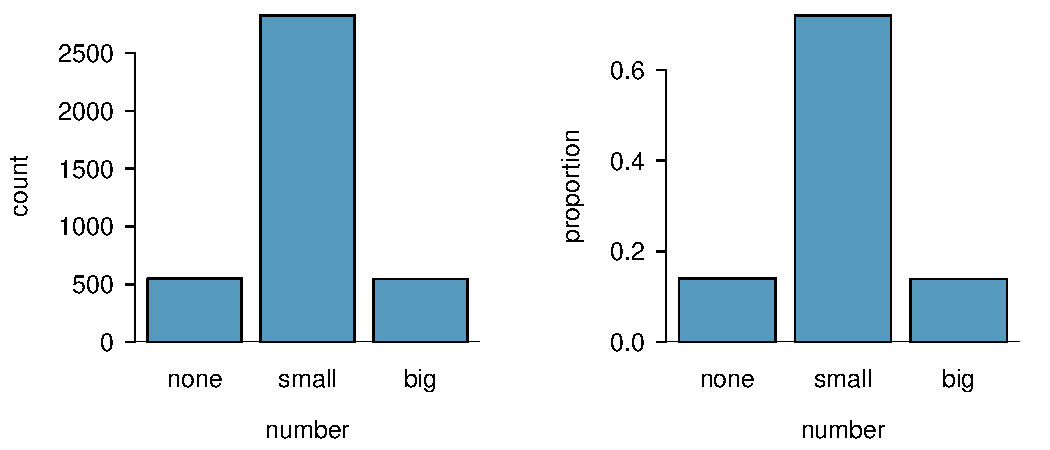
\includegraphics[width=0.9\textwidth]{ch_intro_to_data/figures/emailNumberBarPlot/emailNumberBarPlot}
   \caption{Two bar plots of \var{number}. The left panel shows the counts, and the right panel shows the proportions in each group.}
   \label{emailNumberBarPlot}
\end{figure}


\subsection{Row and column proportions}

Table~\ref{rowPropSpamNumber} shows the row proportions for Table~\ref{emailSpamNumberTableTotals}. The \termsub{row proportions}{contingency table!row proportions} are computed as the counts divided by their row totals. The value 149 at the intersection of \resp{spam} and \resp{none} is replaced by $149/367=0.406$, i.e. 149 divided by its row total, 367. So what does 0.406 represent? It corresponds to the proportion of spam emails in the sample that do not have any numbers.

\begin{table}
\centering
\begin{tabular}{l rrr r}
  \hline
 & none & small & big & Total \\ 
  \hline
spam &  $149/367 = 0.406$ & $168/367 = 0.458$ &
			$50/367 = 0.136$ & 1.000 \\ 
not spam &  $400/3554 = 0.113$ & $2657/3554 = 0.748$ &
			$495/3554 = 0.139$ & 1.000 \\ 
   \hline
Total & $549/3921 = 0.140$ & $2827/3921 = 0.721$ &
			$545/3921 = 0.139$ & 1.000 \\
  \hline
\end{tabular}
\caption{A contingency table with row proportions for the \var{spam} and \var{number} variables.}
\label{rowPropSpamNumber}
% library(openintro); data(email); g <- table(email$spam, email$number)[2:1,]; g / rep(rowSums(g), 3); rowSums(g)
\end{table}

A contingency table of the column proportions is computed in a similar way, where each \termsub{column proportion}{contingency table!column proportion} is computed as the count divided by the corresponding column total. Table~\ref{colPropSpamNumber} shows such a table, and here the value 0.271 indicates that 27.1\% of emails with no numbers were spam. This rate of spam is much higher compared to emails with only small numbers (5.9\%) or big numbers (9.2\%). Because these spam rates vary between the three levels of \var{number} (\resp{none}, \resp{small}, \resp{big}), this provides evidence that the \var{spam} and \var{number} variables are associated.

\begin{table}[h]
\centering\small
\begin{tabular}{l rrr r}
  \hline
 & none & small & big & Total \\ 
  \hline
spam &  $149/549 = 0.271$ & $168/2827 = 0.059$ &
				$50/545 = 0.092$ & $367/3921 = 0.094$ \\ 
not spam &  $400/549 = 0.729$ & $2659/2827 = 0.941$ &
				$495/545 = 0.908$ & $3684/3921 = 0.906$ \\ 
   \hline
Total & 1.000 & 1.000 & 1.000 & 1.000 \\
   \hline
\end{tabular}
\caption{A contingency table with column proportions for the \var{spam} and \var{number} variables.}
\label{colPropSpamNumber}
% library(openintro); data(email); g <- table(email$spam, email$number)[2:1,]; g / rep(colSums(g), rep(2, 3)); g; colSums(g)
\end{table}

We could also have checked for an association between \var{spam} and \var{number} in Table~\ref{rowPropSpamNumber} using row proportions. When comparing these row proportions, we would look down columns to see if the fraction of emails with no numbers, small numbers, and big numbers varied from \resp{spam} to \resp{not~spam}.

\begin{exercise}
What does 0.458 represent in Table~\ref{rowPropSpamNumber}? What does 0.059 represent in Table~\ref{colPropSpamNumber}?\footnote{0.458 represents the proportion of spam emails that had a small number. 0.059 represents the fraction of emails with small numbers that are spam.}
\end{exercise}

\begin{exercise}
What does 0.139 at the intersection of \resp{not~spam} and \resp{big} represent in Table~\ref{rowPropSpamNumber}? What does 0.908 represent in the Table~\ref{colPropSpamNumber}?\footnote{0.139 represents the fraction of non-spam email that had a big number. 0.908 represents the fraction of emails with big numbers that are non-spam emails.}
\end{exercise}

\begin{example}{Data scientists use statistics to filter spam from incoming email messages. By noting specific characteristics of an email, a data scientist may be able to classify some emails as spam or not spam with high accuracy. One of those characteristics is whether the email contains no numbers, small numbers, or big numbers. Another characteristic is whether or not an email has any HTML content. A contingency table for the \var{spam} and \var{format} variables from the \data{email} data set are shown in Table~\ref{emailSpamHTMLTableTotals}. Recall that an HTML email is an email with the capacity for special formatting, e.g. bold text. In Table~\ref{emailSpamHTMLTableTotals}, which would be more helpful to someone hoping to classify email as spam or regular email: row or column proportions?} \label{weighingRowColumnProportions}
Such a person would be interested in how the proportion of spam changes within each email format. This corresponds to column proportions: the proportion of spam in plain text emails and the proportion of spam in HTML emails.

If we generate the column proportions, we can see that a higher fraction of plain text emails are spam ($209/1195 = 17.5\%$) than compared to HTML emails ($158/2726 = 5.8\%$). This information on its own is insufficient to classify an email as spam or not spam, as over 80\% of plain text emails are not spam. Yet, when we carefully combine this information with many other characteristics, such as \var{number} and other variables, we stand a reasonable chance of being able to classify some email as spam or not spam. \GLMSection{This is a topic we will return to in Chapter~\ref{multipleRegressionAndANOVA}.}{}
\end{example}

\begin{table}[ht]
\centering
\begin{tabular}{l cc r}
  \hline
 & text & HTML & Total \\ 
  \hline
spam & 209 & 158 & 367 \\ 
not spam & 986 & 2568 & 3554 \\ 
   \hline
Total & 1195 & 2726 & 3921 \\
   \hline
\end{tabular}
\caption{A contingency table for \var{spam} and \var{format}.}
\label{emailSpamHTMLTableTotals}
%library(openintro); library(xtable); data(email); tab <- table(email[,c("spam", "format")])[2:1,]; tab; colSums(tab); rowSums(tab)
\end{table}

Example~\ref{weighingRowColumnProportions} points out that row and column proportions are not equivalent. Before settling on one form for a table, it is important to consider each to ensure that the most useful table is constructed.

\begin{exercise}
Look back to Tables~\ref{rowPropSpamNumber} and~\ref{colPropSpamNumber}. Which would be more useful to someone hoping to identify spam emails using the \var{number} variable?\footnote{The column proportions in Table~\ref{colPropSpamNumber} will probably be most useful, which makes it easier to see that emails with small numbers are spam about 5.9\% of the time (relatively rare). We would also see that about 27.1\% of emails with no numbers are spam, and 9.2\% of emails with big numbers are spam.}
\end{exercise}


\textC{\newpage}

\subsection{Segmented bar and mosaic plots}
\label{segmentedBarPlotsAndIndependence}

Contingency tables using row or column proportions are especially useful for examining how two categorical variables are related. Segmented bar and mosaic plots provide a way to visualize the information in these tables.

A \termsub{segmented bar plot}{bar plot!segmented bar plot} is a graphical display of contingency table information. For example, a segmented bar plot representing Table~\ref{colPropSpamNumber} is shown in Figure~\ref{emailSpamNumberSegBar}, where we have first created a bar plot using the \var{number} variable and then divided each group by the levels of \var{spam}. The column proportions of Table~\ref{colPropSpamNumber} have been translated into a standardized segmented bar plot in Figure~\ref{emailSpamNumberSegBarSta}, which is a helpful visualization of the fraction of spam emails in each level of \var{number}.

\begin{figure}[h]
\centering
\subfigure[]{
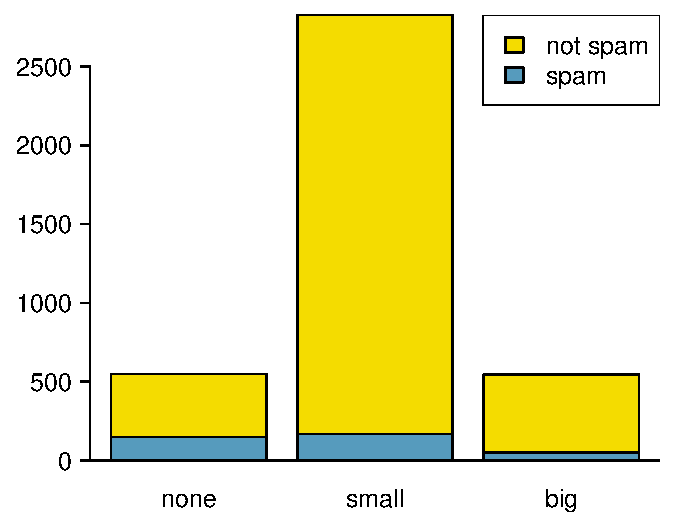
\includegraphics[width=0.46\textwidth]{ch_intro_to_data/figures/emailSpamNumberSegBar/emailSpamNumberSegBar}
\label{emailSpamNumberSegBar}
}
\subfigure[]{
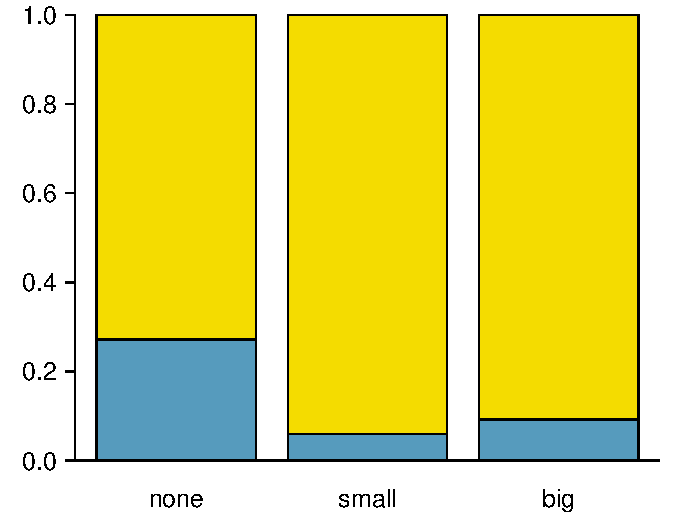
\includegraphics[width=0.46\textwidth]{ch_intro_to_data/figures/emailSpamNumberSegBar/emailSpamNumberSegBarSta}
\label{emailSpamNumberSegBarSta}
}
\caption{\subref{emailSpamNumberSegBar} Segmented bar plot for numbers found in emails, where the counts have been further broken down by \var{spam}. \subref{emailSpamNumberSegBarSta} Standardized version of Figure~\subref{emailSpamNumberSegBar}.}
\label{emailSpamNumberSegBarPlot}
\end{figure}

\begin{example}{Examine both of the segmented bar plots. Which is more useful?}
Figure~\ref{emailSpamNumberSegBar} contains more information, but Figure~\ref{emailSpamNumberSegBarSta} presents the information more clearly. This second plot makes it clear that emails with no number have a relatively high rate of spam email -- about 27\%! On the other hand, less than 10\% of email with small or big numbers are spam.
\end{example}

Since the proportion of spam changes across the groups in Figure~\ref{emailSpamNumberSegBarSta}, we can conclude the variables are dependent, which is something we were also able to discern using table proportions. Because both the \resp{none} and \resp{big} groups have relatively few observations compared to the \resp{small} group, the association is more difficult to see in Figure~\ref{emailSpamNumberSegBar}.

In some other cases, a segmented bar plot that is not standardized will be more useful in communicating important information. Before settling on a particular segmented bar plot, create standardized and non-standardized forms and decide which is more effective at communicating features of the data.

\begin{figure}
\centering
\subfigure[]{
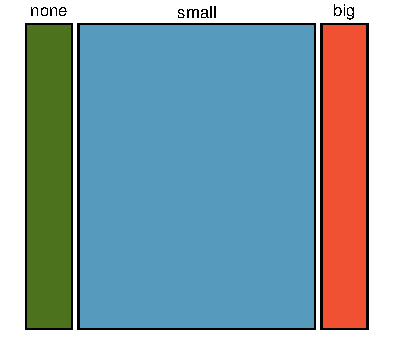
\includegraphics[width=0.3934\textwidth]{ch_intro_to_data/figures/emailSpamNumberMosaicPlot/emailNumberMosaic}
\label{emailNumberMosaic}
}
\subfigure[]{
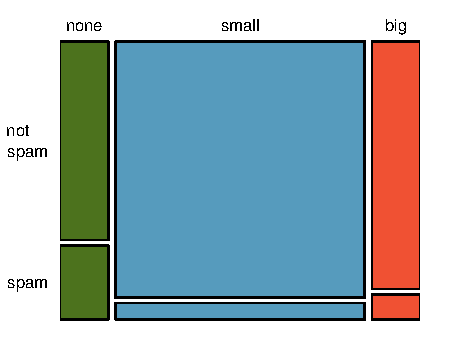
\includegraphics[width=0.46\textwidth]{ch_intro_to_data/figures/emailSpamNumberMosaicPlot/emailSpamNumberMosaic}
\label{emailSpamNumberMosaic}
}
\caption{The one-variable mosaic plot for \var{number} and the two-variable mosaic plot for both \var{number} and \var{spam}.}
\label{emailSpamNumberMosaicPlot}
\end{figure}

A \term{mosaic plot} is a graphical display of contingency table information that is similar to a bar plot for one variable or a segmented bar plot when using two variables. Figure~\ref{emailNumberMosaic} shows a mosaic plot for the \var{number} variable. Each column represents a level of \var{number}, and the column widths correspond to the proportion of emails for each number~type. For~instance, there are fewer emails with no numbers than emails with only small numbers, so the no number email column is slimmer. In general, mosaic plots use box \emph{areas} to represent the number of observations that box represents.

\begin{figure}
   \centering
   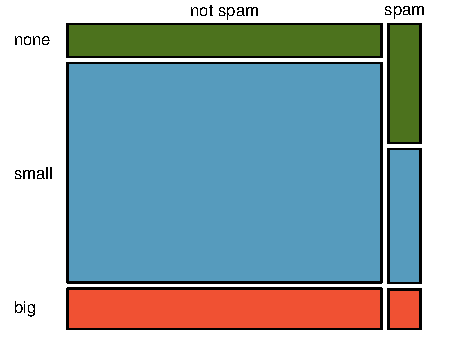
\includegraphics[width=0.44\textwidth]{ch_intro_to_data/figures/emailSpamNumberMosaicPlot/emailSpamNumberMosaicRev}
   \caption{Mosaic plot where emails are grouped by the \var{number} variable after they've been divided into \resp{spam} and \resp{not spam}.}
   \label{emailSpamNumberMosaicRev}
\end{figure}

This one-variable mosaic plot is further divided into pieces in Figure~\ref{emailSpamNumberMosaic} using the \var{spam} variable. Each column is split proportionally according to the fraction of emails that were spam in each number category. For example, the second column, representing emails with only small numbers, was divided into emails that were spam (lower) and not spam (upper). 
As another example, the bottom of the third column represents spam emails that had big numbers, and the upper part of the third column represents regular emails that had big numbers. We can again use this plot to see that the \var{spam} and \var{number} variables are associated since some columns are divided in different vertical locations than others, which was the same technique used for checking an association in the standardized version of the segmented bar plot.

In a similar way, a mosaic plot representing row proportions of Table~\ref{emailSpamNumberTableTotals} could be constructed, as shown in Figure~\ref{emailSpamNumberMosaicRev}. However, because it is more insightful for this application to consider the fraction of spam in each category of the \var{number} variable, we prefer Figure~\ref{emailSpamNumberMosaic}.

\subsection{The only pie chart you will see in this book}

While pie charts are well known, they are not typically as useful as other charts in a data analysis. A \term{pie chart} is shown in Figure~\vref{emailNumberPieChart} alongside a bar plot. It is generally more difficult to compare group sizes in a pie chart than in a bar plot, especially when categories have nearly identical counts or proportions. In the case of the \resp{none} and \resp{big} categories, the difference is so slight you may be unable to distinguish any difference in group sizes for either~plot!

\begin{figure}[h]
   \centering
   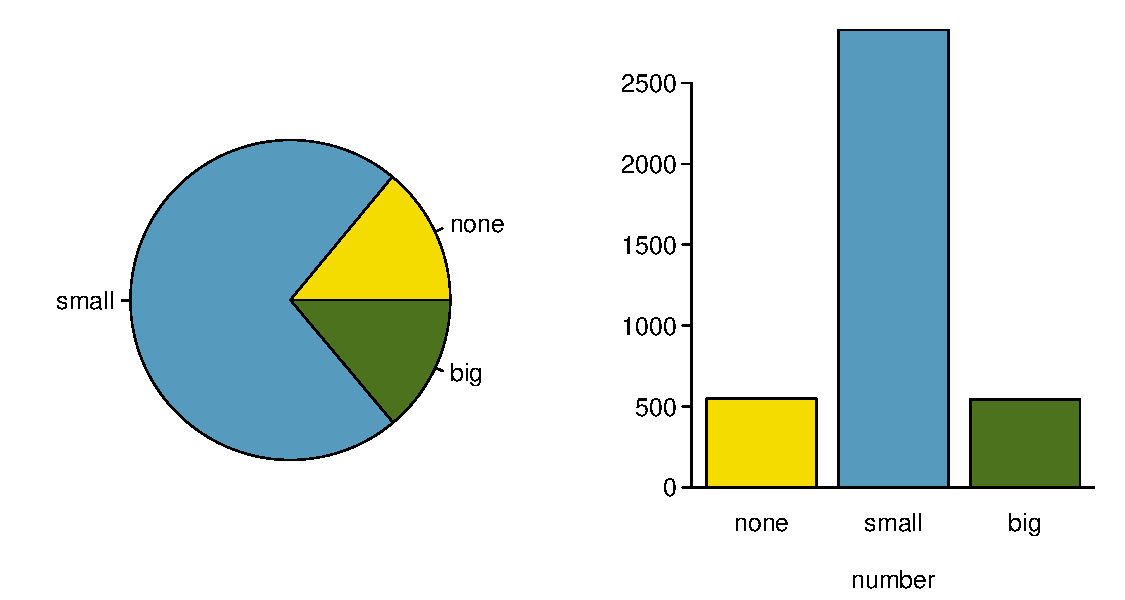
\includegraphics[width=\textwidth]{ch_intro_to_data/figures/emailNumberPieChart/emailNumberPieChart}
   \caption{A pie chart and bar plot of \var{number} for the \data{email} data set.}
   \label{emailNumberPieChart}
\end{figure}

\index{data!email|)}

\subsection{Comparing numerical data across groups}
\label{comparingAcrossGroups}

\index{data!county|(}

Some of the more interesting investigations can be considered by examining numerical data across groups. The methods required here aren't really new. All that is required is to make a numerical plot for each group. Here two convenient methods are introduced: side-by-side box plots and hollow histograms.

We will take a look again at the \data{county} data set and compare the median household income for counties that gained population from 2000 to 2010 versus counties that had no gain. While we might like to make a causal connection here, remember that these are observational data and so such an interpretation would be unjustified.

There were 2,041 counties where the population increased from 2000 to 2010, and there were 1,099 counties with no gain (all but one were a loss). A~random sample of 100 counties from the first group and 50 from the second group are shown in Table~\ref{countyIncomeSplitByPopGainTable} to give a better sense of some of the raw data.

\begin{table}
\centering
\begin{tabular}{ ccc ccc c ccc }
\multicolumn{6}{c}{\bf population gain} && \multicolumn{3}{c}{\bf no gain} \\ 
  \cline{1-6} \cline{8-10}
41.2 & 33.1 & 30.4 & 37.3 & 79.1 & 34.5 &\hspace{5mm}\ & 40.3 & 33.5 & 34.8 \\
22.9 & 39.9 & 31.4 & 45.1 & 50.6 & 59.4 && 29.5 & 31.8 & 41.3 \\
47.9 & 36.4 & 42.2 & 43.2 & 31.8 & 36.9 && 28 & 39.1 & 42.8 \\
50.1 & 27.3 & 37.5 & 53.5 & 26.1 & 57.2 && 38.1 & 39.5 & 22.3 \\
57.4 & 42.6 & 40.6 & 48.8 & 28.1 & 29.4 && 43.3 & 37.5 & 47.1 \\
43.8 & 26 & 33.8 & 35.7 & 38.5 & 42.3 && 43.7 & 36.7 & 36 \\
41.3 & 40.5 & 68.3 & 31 & 46.7 & 30.5 && 35.8 & 38.7 & 39.8 \\
68.3 & 48.3 & 38.7 & 62 & 37.6 & 32.2 && 46 & 42.3 & 48.2 \\
42.6 & 53.6 & 50.7 & 35.1 & 30.6 & 56.8 && 38.6 & 31.9 & 31.1 \\
66.4 & 41.4 & 34.3 & 38.9 & 37.3 & 41.7 && 37.6 & 29.3 & 30.1 \\
51.9 & 83.3 & 46.3 & 48.4 & 40.8 & 42.6 && 57.5 & 32.6 & 31.1 \\
44.5 & 34 & 48.7 & 45.2 & 34.7 & 32.2 && 46.2 & 26.5 & 40.1 \\
39.4 & 38.6 & 40 & 57.3 & 45.2 & 33.1 && 38.4 & 46.7 & 25.9 \\
43.8 & 71.7 & 45.1 & 32.2 & 63.3 & 54.7 && 36.4 & 41.5 & 45.7 \\
71.3 & 36.3 & 36.4 & 41 & 37 & 66.7 && 39.7 & 37 & 37.7 \\
50.2 & 45.8 & 45.7 & 60.2 & 53.1 &  && 21.4 & 29.3 & 50.1 \\
35.8 & 40.4 & 51.5 & 66.4 & 36.1 &  && 43.6 & 39.8 &  \\
\cline{1-6} \cline{8-10}
\end{tabular}
\caption{In this table, median household income (in \$1000s) from a random sample of 100 counties that gained population over 2000-2010 are shown on the left. Median incomes from a random sample of 50 counties that had no population gain are shown on the right.}
\label{countyIncomeSplitByPopGainTable}
\end{table}

The \term{side-by-side box plot} \index{box plot!side-by-side box plot} is a traditional tool for comparing across groups. An example is shown in the left panel of Figure~\ref{countyIncomeSplitByPopGain}, where there are two box plots, one for each group, placed into one plotting window and drawn on the same scale.

\begin{figure}
   \centering
   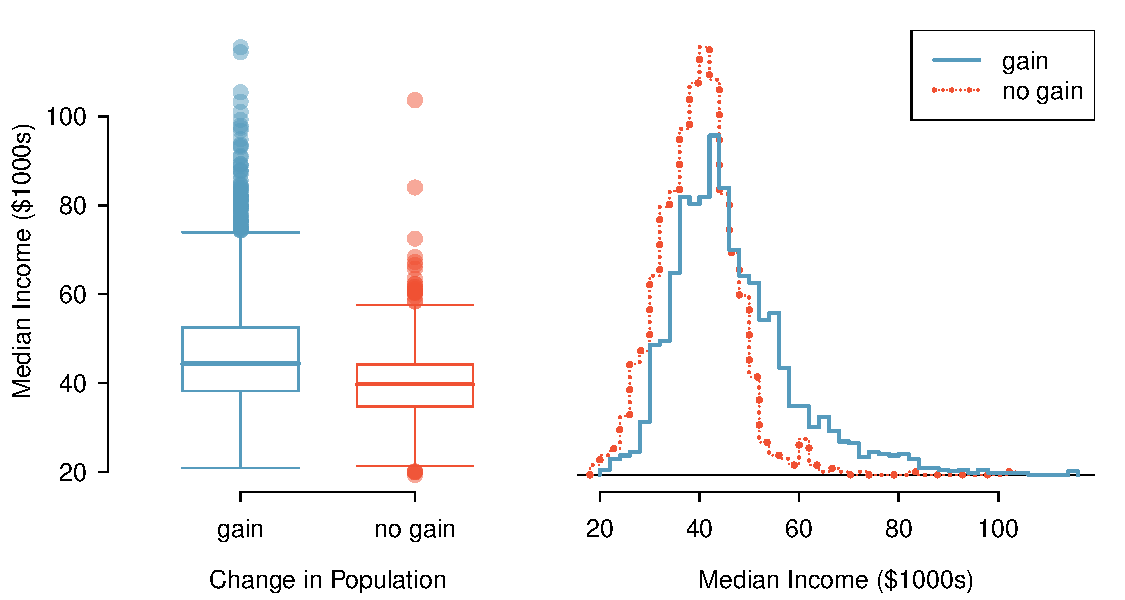
\includegraphics[width=\textwidth]{ch_intro_to_data/figures/countyIncomeSplitByPopGain/countyIncomeSplitByPopGain}
   \caption{Side-by-side box plot (left panel) and hollow histograms (right panel) for \var{med\_\hspace{0.3mm}income}, where the counties are split by whether there was a population gain or loss from 2000 to 2010. The income data were collected between 2006 and 2010.}
   \label{countyIncomeSplitByPopGain}
\end{figure}

Another useful plotting method uses \termsub{hollow histograms}{hollow histogram} to compare numerical data across groups. These are just the outlines of histograms of each group put on the same plot, as shown in the right panel of Figure~\ref{countyIncomeSplitByPopGain}.

\begin{exercise} \label{comparingPriceByTypeExercise}
Use the plots in Figure~\ref{countyIncomeSplitByPopGain} to compare the incomes for counties across the two groups. What do you notice about the approximate center of each group? What do you notice about the variability between groups? Is the shape relatively consistent between groups? How many \emph{prominent} modes are there for each group?\footnote{Answers may vary a little. The counties with population gains tend to have higher income (median of about \$45,000) versus counties without a gain (median of about \$40,000). The variability is also slightly larger for the population gain group. This is evident in the IQR, which is about 50\% bigger in the \emph{gain} group. Both distributions show slight to moderate right skew\index{skew!example: slight to moderate} and are unimodal. There is a secondary small bump at about \$60,000 for the \emph{no gain} group, visible in the hollow histogram plot, that seems out of place. (Looking into the data set, we would find that 8 of these 15 counties are in Alaska and Texas.) The box plots indicate there are many observations far above the median in each group, though we should anticipate that many observations will fall beyond the whiskers when using such a large data set.}
\end{exercise}

\begin{exercise}
What components of each plot in Figure~\ref{countyIncomeSplitByPopGain} do you find most useful?\footnote{Answers will vary. The side-by-side box plots are especially useful for comparing centers and spreads, while the hollow histograms are more useful for seeing distribution shape, skew, and groups of anomalies.}
\end{exercise}

\index{data!county|)}


%___________________________________________
\section[Case study: gender discrimination (special topic)]{Case study: gender discrimination \sectionvideohref{youtube-2pHhjx9hyM4&list=PLkIselvEzpM6pZ76FD3NoCvvgkj_p-dE8} \\(special topic)}
\label{caseStudyGenderDiscrimination}

\index{data!discrimination|(}

\begin{example}{Suppose your professor splits the students in class into two groups: students on the left and students on the right. If $\hat{p}_{_L}$ and $\hat{p}_{_R}$ represent the proportion of students who own an Apple product on the left and right, respectively, would you be surprised if $\hat{p}_{_L}$ did not {exactly} equal $\hat{p}_{_R}$?}\label{classRightLeftSideApple}
While the proportions would probably be close to each other, it would be unusual for them to be exactly the same. We would probably observe a small difference due to {chance}.
\end{example}

\begin{exercise}
If we don't think the side of the room a person sits on in class is related to whether the person owns an Apple product, what assumption are we making about the relationship between these two variables?\footnote{We would be assuming that these two variables are independent.}
\end{exercise}

\subsection{Variability within data}
\label{variabilityWithinData}

We consider a study investigating gender discrimination in the 1970s, which is set in the context of personnel decisions within a bank.\footnote{Rosen B and Jerdee T. 1974. Influence of sex role stereotypes on personnel decisions. Journal of Applied Psychology 59(1):9-14.} The research question we hope to answer is, ``Are females unfairly discriminated against in promotion decisions made by male managers?"

The participants in this study are 48 male bank supervisors attending a management institute at the University of North Carolina in 1972. They were asked to assume the role of the personnel director of a bank and were given a personnel file to judge whether the person should be promoted to a branch manager position. The files given to the participants were identical, except that half of them indicated the candidate was male and the other half indicated the candidate was female. These files were randomly assigned to the subjects.

\begin{exercise}
Is this an observational study or an experiment? What implications does the study type have on what can be inferred from the results?\footnote{The study is an experiment, as subjects were randomly assigned a male file or a female file. Since this is an experiment, the results can be used to evaluate a causal relationship between gender of a candidate and the promotion decision.}
\end{exercise}

For each supervisor we record the gender associated with the assigned file and the promotion decision. Using the results of the study summarized in Table~\ref{discriminationResults}, we would like to evaluate if females are unfairly discriminated against in promotion decisions. In this study, a smaller proportion of females are promoted than males (0.583 versus 0.875), but it is unclear whether the difference provides \emph{convincing evidence} that females are unfairly discriminated against.

\begin{table}[ht]
\centering
\begin{tabular}{l l cc rr}
& & \multicolumn{2}{c}{\var{decision}} \\
  \cline{3-4}
		&			& 	{promoted} 	& {not promoted} & Total & \hspace{3mm}  \\ 
  \cline{2-5}
		&	{male} 			& 21    		& 3   & 24  	 \\ 
  \raisebox{1.5ex}[0pt]{\var{gender}}		&	{female} 	& 14    		& 10     & 24	 \\ 
  \cline{2-5}
  		&	Total		& 35	& 13	&  48 \\
  \cline{2-5}
\end{tabular}
\caption{Summary results for the gender discrimination study.}
\label{discriminationResults}
\end{table}

\begin{example}{Statisticians are sometimes called upon to evaluate the strength of evidence. When looking at the rates of promotion for males and females in this study, what comes to mind as we try to determine whether the data show convincing evidence of a real difference?} \label{discriminationResultsWhatIsConvincingEvidence}
The observed promotion rates (58.3\% for females versus 87.5\% for males) suggest there might be discrimination against women in promotion decisions. However, we cannot be sure if the observed difference represents discrimination or is just from random chance. Generally there is a little bit of fluctuation in sample data, and we wouldn't expect the sample proportions to be \emph{exactly} equal, even if the truth was that the promotion decisions were independent of gender.
\end{example}

Example~\ref{discriminationResultsWhatIsConvincingEvidence} is a reminder that the observed outcomes in the sample may not perfectly reflect the true relationships between variables in the underlying population. Table~\ref{discriminationResults} shows there were 7 fewer promotions in the female group than in the male group, a difference in promotion rates of 29.2\% $\left( \frac{21}{24} - \frac{14}{24} = 0.292 \right)$. This difference is large, but the sample size for the study is small, making it unclear if this observed difference represents discrimination or whether it is simply due to chance. We label these two competing claims, $H_0$ and $H_A$:
\begin{itemize}
\setlength{\itemsep}{0mm}
\item[$H_0$:] \textbf{Independence model.} The variables \var{gender} and \var{decision} are independent. They have no relationship, and the observed difference between the proportion of males and females who were promoted, 29.2\%, was due to chance.
\item[$H_A$:] \textbf{Alternative model.} The variables \var{gender} and \var{decision} are \emph{not} independent. The difference in promotion rates of 29.2\% was not due to chance, and equally qualified females are less likely to be promoted than males.
\end{itemize}

What would it mean if the independence model, which says the variables \var{gender} and \var{decision} are unrelated, is true? It would mean each banker was going to decide whether to promote the candidate without regard to the gender indicated on the file. That~is, the difference in the promotion percentages was due to the way the files were randomly divided to the bankers, and the randomization just happened to give rise to a relatively large difference of 29.2\%.

Consider the alternative model: bankers were influenced by which gender was listed on the personnel file. If this was true, and especially if this influence was substantial, we would expect to see some difference in the promotion rates of male and female candidates. If this gender bias was against females, we would expect a smaller fraction of promotion decisions for female personnel files relative to the male files.

We choose between these two competing claims by assessing if the data conflict so much with $H_0$ that the independence model cannot be deemed reasonable. If this is the case, and the data support $H_A$, then we will reject the notion of independence and conclude there was discrimination.

\subsection{Simulating the study}
\label{simulatingTheStudy}

Table~\ref{discriminationResults} shows that 35 bank supervisors recommended promotion and 13 did not. Now, suppose the bankers' decisions were independent of gender. Then, if we conducted the experiment again with a different random arrangement of files, differences in promotion rates would be based only on random fluctuation. We can actually perform this \term{randomization}, which simulates what would have happened if the bankers' decisions had been independent of gender but we had distributed the files differently.

In this \term{simulation}, we thoroughly shuffle 48 personnel files, 24 labeled \resp{male\_\hspace{0.3mm}sim} and 24 labeled \resp{female\_\hspace{0.3mm}sim}, and deal these files into two stacks. We will deal 35 files into the first stack, which will represent the 35 supervisors who recommended promotion. The second stack will have 13 files, and it will represent the 13 supervisors who recommended against promotion. Then, as we did with the original data, we tabulate the results and determine the fraction of \resp{male\_\hspace{0.3mm}sim} and \resp{female\_\hspace{0.3mm}sim} who were promoted. The randomization of files in this simulation is independent of the promotion decisions, which means any difference in the two fractions is entirely due to chance. Table~\ref{discriminationRand1} show the results of such a simulation.

\begin{table}[ht]
\centering
\begin{tabular}{l l cc rr}
& & \multicolumn{2}{c}{\var{decision}} \\
  \cline{3-4}
		&			& 	{promoted} 	& {not promoted} & Total & \hspace{3mm}  \\ 
  \cline{2-5}
		&	\resp{male\_\hspace{0.3mm}sim} 					& 18    		& 6    & 24 	 \\ 
  \raisebox{1.5ex}[0pt]{\var{gender\_\hspace{0.3mm}sim}}		&	\resp{female\_\hspace{0.3mm}sim} 	& 17    		& 7 & 24    	 \\ 
  \cline{2-5}
  & Total	& 35 & 13 & 48
\end{tabular}
\caption{Simulation results, where any difference in promotion rates between \resp{male\_\hspace{0.3mm}sim} and \resp{female\_\hspace{0.3mm}sim} is purely due to chance.}
\label{discriminationRand1}
\end{table}

\begin{exercise} \label{sampleDifferenceInMaleAndFemaleDiscrimination}
What is the difference in promotion rates between the two simulated groups in Table~\ref{discriminationRand1}? How does this compare to the observed 29.2\% in the actual groups?\footnote{$18/24 - 17/24=0.042$ or about 4.2\% in favor of the men. This difference due to chance is much smaller than the difference observed in the actual groups.}
\end{exercise}


\textC{\pagebreak}

\subsection{Checking for independence}

We computed one possible difference under the independence model in Guided Practice~\ref{sampleDifferenceInMaleAndFemaleDiscrimination}, which represents one difference due to chance. While in this first simulation, we physically dealt out files, it is more efficient to perform this simulation using a computer. Repeating the simulation on a computer, we get another difference due to chance: -0.042. And another: 0.208. And so on until we repeat the simulation enough times that we have a good idea of what represents the \emph{distribution of differences from chance alone}. Figure~\ref{discRandDotPlot} shows a plot of the differences found from 100 simulations, where each dot represents a simulated difference between the proportions of male and female files that were recommended for promotion.

\begin{figure}[ht]
\centering
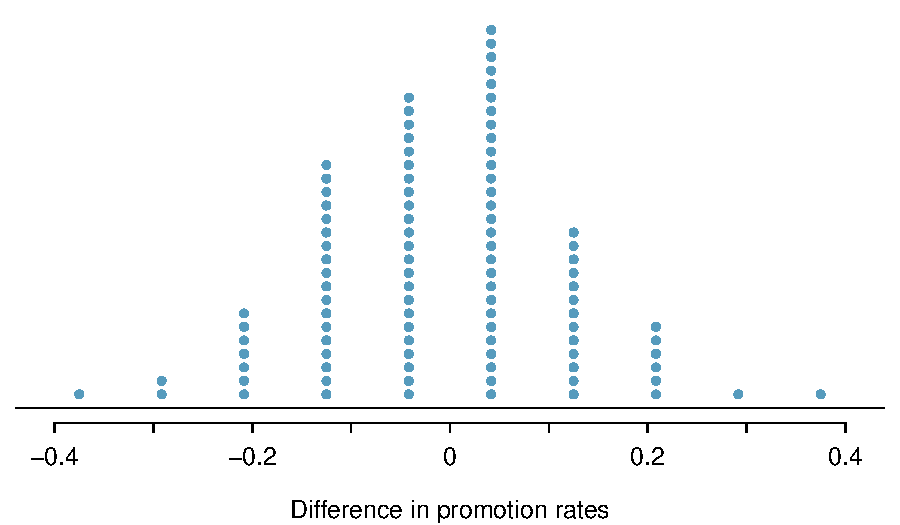
\includegraphics[width=0.85\textwidth]{ch_intro_to_data/figures/discRandDotPlot/discRandDotPlot}
\caption{A stacked dot plot of differences from 100 simulations produced under the independence model, $H_0$, where \var{gender\_\hspace{0.3mm}sim} and \var{decision} are independent. Two of the 100 simulations had a difference of at least 29.2\%, the difference observed in the study.}
\label{discRandDotPlot}
\end{figure}

Note that the distribution of these simulated differences is centered around 0. We simulated these differences assuming that the independence model was true, and under this condition, we expect the difference to be zero with some random fluctuation. We would generally be surprised to see a difference of \emph{exactly} 0: sometimes, just by chance, the difference is higher than 0, and other times it is lower than zero.

\begin{example}{How often would you observe a difference of at least 29.2\% (0.292) according to Figure~\ref{discRandDotPlot}? Often, sometimes, rarely, or never?}
It appears that a difference of at least 29.2\% due to chance alone would only happen about 2\% of the time according to Figure~\ref{discRandDotPlot}. Such a low probability indicates a rare event.
\end{example}

\textC{\newpage}

The difference of 29.2\% being a rare event suggests two possible interpretations of the results of the study:
\begin{itemize}
\setlength{\itemsep}{0mm}
\item[$H_0$] \textbf{Independence model.} Gender has no effect on promotion decision, and we observed a difference that would only happen rarely.
\item[$H_A$] \textbf{Alternative model.} Gender has an effect on promotion decision, and what we observed was actually due to equally qualified women being discriminated against in promotion decisions, which explains the large difference of 29.2\%.
\end{itemize}
Based on the simulations, we have two options. (1)~We conclude that the study results do not provide strong evidence against the independence model. That is, we do not have sufficiently strong evidence to conclude there was gender discrimination. (2)~We conclude the evidence is sufficiently strong to reject $H_0$ and assert that there was gender discrimination. When we conduct formal studies, usually we reject the notion that we just happened to observe a rare event.\footnote{This reasoning does not generally extend to anecdotal observations. Each of us observes incredibly rare events every day, events we could not possibly hope to predict. However, in the non-rigorous setting of anecdotal evidence, almost anything may appear to be a rare event, so the idea of looking for rare events in day-to-day activities is treacherous. For example, we might look at the lottery: there was only a 1 in 176 million chance that the Mega Millions numbers for the largest jackpot in history (March 30, 2012) would be (2, 4, 23, 38, 46) with a Mega ball of (23), but nonetheless those numbers came up! However, no matter what numbers had turned up, they would have had the same incredibly rare odds. That is, \emph{any set of numbers we could have observed would ultimately be incredibly rare}. This type of situation is typical of our daily lives: each possible event in itself seems incredibly rare, but if we consider every alternative, those outcomes are also incredibly rare. We should be cautious not to misinterpret such anecdotal evidence.} So in this case, we reject the independence model in favor of the alternative. That is, we are concluding the data provide strong evidence of gender discrimination against women by the supervisors.

\index{data!discrimination|)}

One field of statistics, statistical inference, is built on evaluating whether such differences are due to chance. In statistical inference, statisticians evaluate which model is most reasonable given the data. Errors do occur, just like rare events, and we might choose the wrong model. While we do not always choose correctly, statistical inference gives us tools to control and evaluate how often these errors occur. In Chapter~\ref{foundationsForInference}, we give a formal introduction to the problem of model selection. We spend the next two chapters building a foundation of probability and theory necessary to make that discussion rigorous.
